
\clearpage
\pageoriginale

\SGAExposeBookmark{XIV}{Comparación con la teoría trascendente}
\begin{center}
{\large\textbf{SGA 7}}\\[1.5em]
{\Large\underline{EXPOSÉ XIV}}\\[2.5em]
{\Large\underline{COMPARACIÓN CON LA TEORÍA TRASCENDENTE}}\\[1.5em]
{\large\underline{por P. DELIGNE}}
\end{center}

\bigskip
\noindent\textbf{Índice de la fuente}
\begin{center}
\begin{tabular}{@{}llr@{}}
Introducción && 1\\
\S1. & Formalismo trascendente de los ciclos evanescentes & 1\\
1.1 & Grupo fundamental del disco perforado: convenciones de signos & 2\\
1.2 & Haces de conjuntos & 5\\
1.3 & El funtor $R\Psi$ & 10\\
1.4 & Un caso particular & 12\\
\S2. & El teorema de comparación & 16\\
\S3. & Singularidades aisladas & 20\\
3.1 & La variedad de los ciclos evanescentes & 20\\
3.2 & La fórmula de Picard--Lefschetz (caso trascendente) & 31\\
\S4. & Cohomología de De Rham & 38
\end{tabular}
\end{center}

\medskip
\noindent\underline{Introducción}

Para comparar la teoría de los ciclos evanescentes del Exposé XIII con su
análogo trascendente sobre $\mathbb C$, procederemos en dos etapas.

\begin{enumerate}[label=(\alph*),leftmargin=2.6em]
\item Daremos un formalismo trascendente modelado sobre el del Exposé XIII y
demostraremos un teorema de comparación por los métodos habituales (ya
utilizados para demostrar el teorema de finitud en XIII, 2.3).

\item En el caso de singularidades aisladas, explicitaremos en términos más
concretos el significado del formalismo trascendente aquí introducido.
\end{enumerate}

Además del teorema de comparación, esta exposición contiene una demostración de
la fórmula de Picard--Lefschetz en el caso trascendente.

\pageoriginale

En el §4 damos un resultado preliminar para la teoría de Hodge de los ciclos
evanescentes. Esa sección no se utilizará en lo que sigue del seminario.

\section*{1. Formalismo trascendente de los ciclos evanescentes}

\subsection*{1.1. El grupo fundamental del disco perforado: convenciones de
signos}

Tendremos que considerar discos perforados $D^*$ y su grupo fundamental
$\mathbb Z$. Como este grupo es abeliano, pueden aparecer ambigüedades de
signo. Las eliminamos olvidando que es abeliano.

\subsubsection*{1.1.1.}
Sea $X$ un buen espacio topológico conexo y sea $x\in X$. Los elementos del
grupo fundamental son las clases de homotopía de lazos con punto base $x$. Si
$\alpha,\beta\in\pi_1(X,x)$ están representados por los lazos $a,b$, entonces
$\alpha\beta$ está representado por el lazo que se obtiene recorriendo primero
$b$ y después $a$.

\subsubsection*{1.1.2.}
Sea $F$ un haz localmente constante sobre $X$. Para todo camino
$a:[0,1]\longrightarrow X$, la imagen inversa $a^*F$ sobre $[0,1]$ es
localmente constante y, por tanto, constante, de donde resulta una biyección
\[
a:F_{a(0)}
\xleftarrow{\ \sim\ }H^0([0,1],a^*F)
\xrightarrow{\ \sim\ }F_{a(1)}.
\]
Esta biyección solo depende de la clase de homotopía de $a$. Mediante esta
construcción, $\pi_1(X,x)$ actúa por la izquierda sobre $F_x$. El funtor
$F\longmapsto F_x$ es una equivalencia de la categoría de los haces localmente
constantes sobre $X$ con la categoría de los conjuntos provistos de una acción
de $\pi_1(X,x)$.

\subsubsection*{1.1.3.}
Cuando $x$ varía, los grupos $\pi_1(X,x)$ son las fibras de un haz de grupos
localmente constante $\Pi_1(X)$, que actúa sobre todo haz localmente constante
$F$. Si $\pi_1(X,x)$ es abeliano, entonces $\Pi_1(X)$ es constante; su valor
se denota por $\pi_1(X)$.

\subsubsection*{1.1.4.}
El grupo $\pi_1(X,x)$ actúa sobre el recubrimiento universal
\[
p:(\widetilde X,\widetilde x)\longrightarrow(X,x).
\]
Considerado como un espacio étalé sobre $X$, y por tanto como un haz (el haz de
sus secciones locales), este recubrimiento corresponde por 1.1.2 al conjunto
$\pi_1(X,x)$ con elemento distinguido $e$, sobre el cual $\pi_1(X,x)$ actúa
por traslación a izquierda.

\pageoriginale

El grupo actúa también sobre este $\pi_1$-conjunto por automorfismos de
$\pi_1$-conjuntos: un elemento $\sigma\in\pi_1(X,x)$ actúa mediante
\[
g\longmapsto g\sigma^{-1}.
\]
Esta construcción identifica
\[
\pi_1(X,x)=\operatorname{Aut}_X(\widetilde X).
\]

Si $F$ es localmente constante sobre $X$, la biyección
\begin{equation}\tag{1.1.4.1}
H^0(\widetilde X,p^*F)
\longrightarrow(p^*F)_{\widetilde x}=F_x
\end{equation}
conmuta con la acción de $\pi_1(X,x)$: a la izquierda, la acción es el
transporte de estructura mediante su acción sobre $\widetilde X$; a la
derecha, es la acción de 1.1.2. La equivalencia de 1.1.2 puede reformularse,
por tanto, diciendo que
\[
F\longmapsto
\bigl(\widetilde X\longmapsto H^0(\widetilde X,p^*F)\bigr)
\]
es una equivalencia de la categoría de los haces localmente constantes sobre
$X$ con la categoría de los funtores
\[
(\text{recubrimientos universales de }X)\longrightarrow(\text{Conjuntos}).
\]

\subsubsection*{1.1.5.}
Si $\pi_1(X,x)$ es abeliano y, por tanto, independiente de $x$, la acción de
1.1.4 de $\pi_1(X)$ sobre $\widetilde X$ es independiente del punto base:
$\pi_1(X)$ actúa sobre todo recubrimiento universal $\widetilde X$ de $X$.

Hay que tener presente que esta acción, que es la única que utilizaremos,
corresponde a la inversa de la acción de 1.1.3.

\subsubsection*{1.1.6.}
Sea $D$ un disco, es decir, un espacio topológico homeomorfo al disco estándar
\[
\{z\in\mathbb C:|z|<1\}.
\]
Sea $0\in D$ y pongamos $D^*=D\setminus\{0\}$. Supongamos que $D$ está
provisto de una estructura de variedad analítica y, por tanto, orientado. El
grupo fundamental $\pi_1(D^*)$ es entonces canónicamente isomorfo a
$\mathbb Z$. Para el disco estándar, de centro $0$, y $t\in D^*$, el
generador positivo de $\pi_1(D^*,t)$ está representado por el lazo
\[
x\longmapsto \exp(2\pi i x)t.
\]

\subsubsection*{1.1.7.}
Sea $z:D\longrightarrow\mathbb C$ un parámetro uniformizante, de modo que
$(dz)_0\ne0$, y sea $\widetilde D^*$ un recubrimiento universal de $D^*$.
Denotemos por $\log z$ una función cualquiera sobre $\widetilde D^*$ tal que
\[
\exp(\log z)=z.
\]

\pageoriginale

El par $(\widetilde D^*,\log z)$ es único salvo isomorfismo único.

Para $\alpha\in\mathbb C$, pongamos
\[
z^\alpha=\exp(\alpha\log z).
\]
Sea $T$ el generador positivo de $\pi_1(D^*)$, que actúa sobre
$\widetilde D^*$ como en 1.1.5 y sobre las funciones de $\widetilde D^*$ por
transporte de estructura. Entonces
\begin{equation}\tag{1.1.7.1}
T\log z=\log z+2\pi i,
\end{equation}
y
\begin{equation}\tag{1.1.7.2}
Tz^\alpha=\exp(2\pi i\alpha)z^\alpha.
\end{equation}

\subsubsection*{1.1.8.}
Sea $D$ un disco, sea $0\in D$, y pongamos $D^*=D\setminus\{0\}$. Si
$D'\subset D$ es un disco más pequeño que contiene $0$, la restricción a
$D'^*$ es una equivalencia de la categoría de los haces localmente constantes
sobre $D^*$ con la categoría de los haces localmente constantes sobre $D'^*$.
En efecto, para $t\in D'^*$,
\[
\pi_1(D'^*,t)\xrightarrow{\ \sim\ }\pi_1(D^*,t).
\]

Supongamos ahora que $D$ está provisto de una estructura de variedad
diferenciable. Sea $T$ el espacio tangente a $D$ en $0$, y pongamos
$T^*=T\setminus\{0\}$. Para $D'\subset D$ como arriba y una inmersión
$f:D'\hookrightarrow T$ que satisface $f(0)=0$ y $(df)_0=\mathrm{id}$, el
compuesto
\[
(\text{restricción a }D')^{-1}\circ f^*
\]
es una equivalencia $[f]$ de la categoría de los haces localmente constantes
sobre $T^*$ con la categoría de los haces localmente constantes sobre $D^*$.
Salvo isomorfismo canónico, solo depende del germen de $f$ en $0$, sujeto a
$(df)_0=\mathrm{id}$. Un camino de un germen de este tipo a otro define un
isomorfismo de equivalencias, y los caminos homotópicos definen el mismo
isomorfismo. Como el espacio de tales gérmenes es contráctil ---mediante la
retracción a un germen fijo $f_0$ dada por
$(1-\lambda)f+\lambda f_0$---, se obtiene una equivalencia, bien definida
salvo isomorfismo único, de los haces localmente constantes sobre $T^*$ con
los haces localmente constantes sobre $D^*$.

\subsubsection*{1.1.9.}
Sea $D$ un disco, sea $0\in D$, pongamos $D^*=D\setminus\{0\}$, y sea
$p:\widetilde D^*\longrightarrow D^*$ un recubrimiento universal. Escribimos
\[
p:\widetilde D\longrightarrow D
\]
para el espacio topológico sobre $D$ obtenido de $\widetilde D^*$ añadiendo
un punto $0$, de modo que:

\pageoriginale

\begin{enumerate}[label=(\alph*),leftmargin=2.6em]
\item $\widetilde D^*$ es abierto en $\widetilde D$;
\item $p:\widetilde D\longrightarrow D$ prolonga
$p:\widetilde D^*\longrightarrow D^*$ y $p(0)=0$;
\item los conjuntos $p^{-1}(U)$, cuando $U$ recorre los entornos de $0$ en
$D$, forman una base de entornos de $0$ en $\widetilde D$.
\end{enumerate}

\subsubsection*{1.1.10.}
Sea $X$ una curva algebraica compleja no singular, sea $0\in X$, y sea $D$
un entorno disco de $0$ en $X$. El anillo de gérmenes en $0$ de funciones
holomorfas sobre $D$ algebraicas sobre el cuerpo $K(X)$ de funciones
racionales de $X$ es el henselizado $\mathcal O_0^h$ del anillo local
$\mathcal O_0$ de $X$ en $0$. Sea $\widetilde D^*$ un recubrimiento universal
de $D^*=D\setminus\{0\}$. El cuerpo de gérmenes en $0\in\widetilde D$ de
funciones meromorfas sobre $\widetilde D^*$ algebraicas sobre $K(X)$ es una
clausura algebraica $\overline K$ de $K(X)$ y, por tanto, también del cuerpo
de fracciones $K_0^h$ de $\mathcal O_0^h$.

El grupo $\pi_1(D^*)$ de $D$-automorfismos de $\widetilde D^*$ (1.1.5)
actúa por transporte de estructura sobre $\overline K$, dando
\begin{equation}\tag{1.1.10.1}
\begin{tikzcd}[column sep=huge, row sep=large]
\pi_1(D^*) \arrow[r] \arrow[d, equal]
  & \operatorname{Gal}(\overline K/K_0^h) \arrow[d, equal]
  & {} \\
\mathbb Z
  & \widehat{\mathbb Z}(1)
  & .
\end{tikzcd}
\end{equation}
De (1.1.7.2) se sigue que este diagrama es compatible con la inclusión natural,
sobre $\mathbb C$, de $\mathbb Z$ en $\widehat{\mathbb Z}(1)$. Esta inclusión
es el compuesto de $\mathbb Z\hookrightarrow\widehat{\mathbb Z}$ y el
isomorfismo
\[
\widehat{\mathbb Z}\xrightarrow{\ \sim\ }
\widehat{\mathbb Z}(1),
\]
que es el límite inverso de los isomorfismos
\[
\mathbb Z/n\longrightarrow\mu_n,
\qquad
k\longmapsto\exp\left(\frac{2\pi i}{n}k\right).
\]

\subsubsection*{1.1.11.}
Todo haz $F$ sobre $\operatorname{Spec}(K_0^h)$ define un haz localmente
constante sobre $D^*$. Utilizamos la equivalencia de 1.1.4 y, a cada
recubrimiento universal $\widetilde D^*$ de $D^*$, asociamos
$F_{\overline K}$ para el cuerpo $\overline K$ construido en 1.1.10.

\subsection*{1.2. Haces de conjuntos}

\subsubsection*{1.2.1.}
Sea $D$ un disco (1.1.6), sea $0\in D$, y pongamos
$D^*=D\setminus\{0\}$. Denotamos por $\mathcal D^*$ el topos de los haces de
conjuntos localmente constantes sobre $D^*$.

\pageoriginale

Por 1.1.8, este topos no «cambia» si se reemplaza $D$ por un disco más pequeño
$D'$ que contenga $0$, ni, cuando $D$ está provisto de una estructura de
variedad diferenciable, si se reemplaza $D$ por su espacio tangente en $0$.

Para $t\in D^*$, el funtor $F\longmapsto F_t$ identifica este topos con el
topos de los conjuntos provistos de una acción de $\pi_1(D^*)$ (1.1.2). Por
1.1.4, el funtor
\[
F\longmapsto
\bigl(\widetilde D^*\longmapsto
H^0(\widetilde D^*,p^*F)\bigr)
\]
lo identifica con el topos de los funtores
\[
(\text{recubrimientos universales de }D^*)
\longrightarrow(\text{Conjuntos}),
\]
y estas identificaciones están relacionadas por (1.1.4.1).

\subsubsection*{1.2.2.}
Sea $F$ un haz sobre $D$ cuya restricción a $D^*$ es localmente constante.
Existe un único morfismo de haces
\[
\underline{F_0}\xrightarrow{\ \alpha\ }F
\]
cuya aplicación sobre el tallo en $0$ es la identidad. Como se explicó en
XIII, 0.1 (con $X_0=(P^t)$), el funtor
\[
F\longmapsto(F_0,F|_{D^*},\alpha)
\]
identifica estos haces con las ternas formadas por un conjunto $F_0$, un haz
localmente constante $F_\eta$ sobre $D^*$ y un morfismo
\[
\alpha:
(\text{haz constante de valor }F_0\text{ sobre }D^*)
\longrightarrow F_\eta.
\]

\subsubsection*{1.2.3.}
Denotamos por $\mathcal D$ el topos de los haces de conjuntos sobre $D$ cuya
restricción a $D^*$ es localmente constante. La inclusión de $\mathcal D$ en
el topos de los haces sobre $D$ es el funtor imagen inversa de un morfismo de
topoi $D\longrightarrow\mathcal D$, que forma parte del diagrama conmutativo
\[
\begin{tikzcd}
\{0\} \arrow[r, hook] \arrow[d, equal]
  & D \arrow[d, "\beta"]
  & D^* \arrow[l, hook'] \arrow[d, "\beta"] & {} \\
\{0\} \arrow[r, hook]
  & \mathcal D
  & \mathcal D^* \arrow[l, hook'] & {}.
\end{tikzcd}
\]
Como en 1.1.1, se comprueba que este topos no cambia cuando se reemplaza $D$
por un disco más pequeño o por el espacio tangente a $D$ en $0$.

\pageoriginale

\subsubsection*{1.2.4.}
Sea $Y$ un espacio topológico. El topos producto $Y\times\mathcal D$ posee las
tres descripciones siguientes (para su equivalencia, véase XIII, 0.1).

\medskip
\noindent\textit{(a)} $Y\times\mathcal D$ es el topos de los haces $F$ sobre
$Y\times D$ que satisfacen

\smallskip
\noindent $(*)$ $D^*$ está recubierto por abiertos $U$ tales que
$F|_{Y\times U}$ es la imagen inversa de un haz sobre $Y$.

\medskip
\noindent\textit{(b)} Sea $t\in D^*$. El topos $Y\times\mathcal D$ es el
topos de las ternas $(F_0,F_t,\alpha)$ en las que

\smallskip
\noindent $\alpha)$ $F_0$ es un haz sobre $Y$;

\noindent $\beta)$ $F_t$ es un haz sobre $Y$ provisto de una acción de
$\pi_1(D^*)$;

\noindent $\gamma)$ $\alpha:F_0\longrightarrow F_t$ es un morfismo cuya
imagen está contenida en los invariantes.

\medskip
\noindent\textit{(c)} El topos $Y\times\mathcal D$ es el topos de las ternas
$(F_0,F_\eta,\alpha)$ en las que

\smallskip
\noindent $\alpha')$ $F_0$ es un haz sobre $Y$;

\noindent $\beta')$ $F_\eta$ es un funtor, cuyos valores se denotan por
$F_{\bar\eta}$,
\[
(\text{recubrimientos universales de }D^*)
\longrightarrow(\text{haces sobre }Y);
\]

\noindent $\gamma')$ $\alpha$ es un morfismo de $F_0$ (considerado como el
funtor constante de valor $F_0$ de los recubrimientos universales de $D^*$ a
los haces sobre $Y$) a $F_\eta$.

No importa aquí que este topos sea literalmente el topos producto de $Y$ y
$\mathcal D$. Análogamente, definimos $Y\times\mathcal D^*$, a nuestra
elección, como

\medskip
\noindent\textit{(a$^*$)} el topos de los haces sobre $Y\times D^*$ que
satisfacen $(*)$;

\noindent\textit{(b$^*$)} para $t\in D^*$, el topos de los haces $F_t$ sobre
$Y$ provistos de una acción de $\pi_1(D^*)$;

\noindent\textit{(c$^*$)} el topos de los funtores
\[
(\text{recubrimientos universales de }D^*)
\longrightarrow(\text{haces sobre }Y).
\]

\subsubsection*{1.2.5.}
El topos $Y\times\mathcal D$ posee las mismas propiedades de funtorialidad en
$Y$ que los topoi $Y\times_S S$ del Exposé XIII, y no las enumeraremos. Para
fijar la notación, registramos únicamente el diagrama

\pageoriginale

\[
\begin{tikzcd}[row sep=huge, column sep=huge]
Y \arrow[d, ""{name=A}]
  & Y \arrow[d, ""{name=B}] \arrow[r, hook, "i"]
  & Y\times\mathcal D \arrow[d]
  & Y\times\mathcal D^* \arrow[d] \arrow[l, hook', "j"'] \\
(P^t)
  & \{0\} \arrow[r, hook, "i"]
  & \mathcal D
  & \mathcal D^* \arrow[l, hook', "j"']
    \arrow[from=B, to=A, "\mathrm{sp}"']
\end{tikzcd}
\]

\subsubsection*{1.2.6.}
Sea $K$ un complejo de haces de grupos abelianos sobre
$Y\times\mathcal D$. Como en XIII, 1.4.2, se obtiene de $K$ un triángulo
distinguido en $K(Y\times\mathcal D^*)$:
\[
\begin{tikzcd}[row sep=large, column sep=large]
{} & \Phi(K) \arrow[dl] & {} \\
\mathrm{sp}^*K_0 \arrow[rr] & {} & K_\eta \arrow[ul]
\end{tikzcd}
\]
Esta construcción pasa a la categoría derivada y define un funtor
\[
D(Y\times\mathcal D)
\longrightarrow
(\text{triángulos distinguidos de }D(Y\times\mathcal D^*)).
\]

Supongamos que $D$ está orientado (por ejemplo, que es analítico complejo), y
sea $T$ el generador positivo de $\pi_1(D^*)$ (1.1.6). Para
$K\in\operatorname{Ob}D(Y\times\mathcal D)$ definimos, como en XIII, 1.4.3,
la \underline{variación} $V=\operatorname{Var}(T)$,
\[
V:\Phi(K)\longrightarrow K_\eta.
\]
El endomorfismo $T-\mathrm{Id}$ de $K_\eta$ es el compuesto
\[
T-\mathrm{Id}:K_\eta\longrightarrow\Phi(K)
\longrightarrow K_\eta.
\]

\subsubsection*{1.2.7.}
Sea $D$ un disco, sea $0\in D$, pongamos $D^*=D\setminus\{0\}$, sea
$f:X\longrightarrow D$ una aplicación continua, y pongamos
$X_0=f^{-1}(0)$. Definiremos un funtor
\[
\Psi:(\text{haces sobre }X)
\longrightarrow(\text{haces sobre }X_0\times\mathcal D).
\]
Sea $\widetilde D^*$ un recubrimiento universal de $D^*$, sea
$\widetilde D$ como en 1.1.9, y pongamos

\pageoriginale

\[
\overline X=X\times_D\widetilde D,
\qquad
X^*=X\setminus X_0=X\times_DD^*,
\qquad
\overline X^*=\overline X\setminus X_0=X\times_D\widetilde D^*.
\]
Se tiene un diagrama conmutativo
\begin{equation}\tag{1.2.7.1}
\begin{tikzcd}
X_0 \arrow[r, hook, "\overline i"] \arrow[d, equal]
  & \overline X \arrow[d, "p"]
  & \sisi{X^*}{\overline X^*} \arrow[l, hook, "\overline j"']
      \arrow[d, "p'"] \\
X_0 \arrow[r, hook, "i"]
  & X
  & X^* \arrow[l, hook, "j"']
\end{tikzcd}
\end{equation}
cartesiano sobre el diagrama
\begin{equation}\tag{1.2.7.2}
\begin{tikzcd}
\{0\} \arrow[r, hook, "\overline i"] \arrow[d, equal]
  & \widetilde D \arrow[d, "p"]
  & \widetilde D^* \arrow[l, hook, "\overline j"']
      \arrow[d, "p'"] \\
\{0\} \arrow[r, hook, "i"]
  & D
  & D^* \arrow[l, hook, "j"']
\end{tikzcd}
\end{equation}
\noindent\emph{Nota editorial.} En (1.2.7.1), el nodo superior derecho
impreso carece de barra. La definición precedente y la aplicación $p'$ obligan
a que ese nodo sea $\overline X^*$, notación utilizada en la rama corregida.

Para un haz $F$ sobre $X$, ponemos (con la notación de 1.2.4(c))
\[
\Psi(F)=
\bigl(i^*F,\ \overline i^*\overline j_*((jp')^*F),\ \alpha\bigr),
\]
donde
\[
\begin{split}
\alpha:i^*F=\overline i^*p^*F
&\longrightarrow
\overline i^*\overline j_*((jp')^*F)\\
&=\overline i^*\overline j_*\overline j^*p^*F
\end{split}
\]
se obtiene, después de aplicar $\overline i^*$, de la aplicación de adjunción
$\mathrm{Id}\longrightarrow\overline j_*\overline j^*$.

Definimos también un funtor
\[
\Psi_\eta:(\text{haces sobre }X^*)
\longrightarrow(\text{haces sobre }X_0\times\mathcal D^*)
\]
mediante
\[
\Psi_\eta(F)=\overline i^*\overline j_*({p'}^*F).
\]

\subsubsection*{1.2.8.}
Las propiedades de funtorialidad de $\Psi$ son las mismas que las de su
análogo estudiado en XIII, 1.3.5--1.3.9.

\pageoriginale

\subsection*{\texorpdfstring{1.3. El funtor $R\Psi$}{1.3. El funtor R Psi}}

\subsubsection*{1.3.1.}
Sea $D$ un disco, sea $0\in D$, pongamos $D^*=D\setminus\{0\}$, sea
$f:X\longrightarrow D$ una aplicación continua, y pongamos
$X_0=f^{-1}(0)$. Los funtores $R\Psi$ y $R\Psi_\eta$ son los funtores
derivados de $\Psi$ y $\Psi_\eta$:
\[
R\Psi:D^+(X)\longrightarrow D^+(X_0\times\mathcal D),
\]
\[
R\Psi_\eta:D^+(X^*)\longrightarrow D^+(X_0\times\mathcal D^*).
\]
Denotamos por $R\Phi$ el funtor compuesto $\Phi\circ R\Psi$:
\[
R\Phi:D^+(X)\longrightarrow D^+(X_0\times\mathcal D^*).
\]
Las propiedades de estos funtores son exactamente análogas a las de los
funtores del mismo nombre de XIII, 2.1. Sus demostraciones son mucho más
elementales, pues en el marco topológico son fáciles de demostrar los teoremas
de cambio de base para un morfismo propio o para un morfismo liso (es decir,
localmente isomorfo a $\mathbb R^n\times S\longrightarrow S$). Las pequeñas
modificaciones necesarias son las siguientes.

\subsubsection*{1.3.2.}
El funtor $Rf_!$ solo se define para un morfismo separado entre espacios
localmente compactos, y es el funtor derivado del funtor imagen directa con
soportes propios $f_!$.

\subsubsection*{1.3.3.}
Para un morfismo propio (y separado) $f:X\longrightarrow D$, el isomorfismo
fundamental (XIII, (2.1.8.3)) debe reescribirse como sigue. Sea
$p:\widetilde D^*\longrightarrow D^*$ un recubrimiento universal de $D^*$.
Para todo entorno $U$ de $0$ en $D$, pongamos
\[
\widetilde U^*=p^{-1}(U),
\qquad
X_{\widetilde U^*}=X\times_D\widetilde U^*.
\]
Para $K\in\operatorname{Ob}D^+(f^{-1}(D^*))$, se tiene
\begin{equation}\tag{1.3.3.1}
\varinjlim_U\mathbb H^i(X_{\widetilde U^*},K)
\xrightarrow{\ \sim\ }
\mathbb H^i(X_0,R\Psi_{\bar\eta}(K)).
\end{equation}
Este isomorfismo es especialmente útil cuando $X^*=f^{-1}(D^*)$ es un fibrado
topológico sobre $D^*$. Al contraerse hacia $0$ un disco $U\subset D$, la
sucesión espectral de Leray de
$X_{\widetilde U^*}\longrightarrow\widetilde U^*$ muestra entonces que, para
todo haz localmente constante $\Lambda$ sobre $X^*$ y todo
$t\in\widetilde U^*$,
\[
H^i(X_{\widetilde U^*},\Lambda)
\xrightarrow{\ \sim\ }H^i(X_t,\Lambda).
\]

\pageoriginale

Así, para $t\in D^*$,
\begin{equation}\tag{1.3.3.2}
H^i(X_t,\Lambda)
\xrightarrow{\ \sim\ }
H^i(X_0,R\Psi_t(\Lambda)),
\end{equation}
siempre que $X/D$ sea propio, $X^*$ sea un fibrado y $\Lambda$ sea localmente
constante.

En la práctica, para verificar que $X^*$ es un fibrado sobre $D^*$ se utiliza
el teorema de isotopía de Thom, una de cuyas formas se enuncia a continuación.
Para la demostración de este teorema, ninguna de cuyas consecuencias se
utilizará en las exposiciones posteriores, remitimos a Whitney y Mather.

\subsubsection*{1.3.4. Preliminar.}
Sea $f:X\longrightarrow Y$ un morfismo liso (por definición, sin puntos
críticos) de variedades diferenciables. Una \underline{conexión} $\nabla$
sobre $X/Y$ es un subfibrado vectorial del fibrado tangente de $X$
complementario de $\ker(df)$. Para un campo vectorial $u$ sobre $Y$, existe un
único campo vectorial $\nabla(u)$ sobre $X$ que levanta $u$ y pertenece a este
subfibrado. La conexión se llama integrable si
\[
\nabla([u,v])=[\nabla(u),\nabla(v)].
\]
Cuando $f$ es propio, una conexión integrable proporciona trivializaciones
locales sobre $Y$ de $X/Y$,
\[
\alpha:f^{-1}(U)\xrightarrow{\ \sim\ }X_0\times U,
\]
compatibles con la proyección sobre $U$ y que satisfacen
$d\alpha(\nabla(u))=(0,u)$. Cuando $f$ no es propio, el mismo resultado es
válido bajo condiciones adecuadas en el infinito; por ejemplo, basta con que
$\nabla(u)g$ se anule para una función de agotamiento conveniente $g$.

\subsubsection*{1.3.5. Teorema de isotopía de Thom.}
\textit{Sean
\[
D=\{z\in\mathbb C:|z|<1\},
\qquad D^*=D\setminus\{0\},
\]
y sea $f:X\longrightarrow D$ un morfismo propio de espacios analíticos. Tras
reemplazar $D$ por un disco más pequeño y $X$ por su imagen inversa, existe
una estratificación $\Sigma$ de $X^*=f^{-1}(D^*)$ con las propiedades
siguientes:}

\begin{enumerate}[label=(\alph*),leftmargin=2.7em]
\item \textit{$\Sigma$ es una filtración
\[
X^*=F_0\supset F_1\supset\cdots\supset F_n
\supset F_{n+1}=\varnothing
\]
de $X^*$ por subconjuntos cerrados, tal que la clausura $\overline F_i$ de
$F_i$ en $X$ es un subespacio analítico de $X$.}

\pageoriginale

\item \textit{Los estratos abiertos $F_i-F_{i+1}$ son lisos sobre $D^*$.}

\item \textit{$\Sigma$ satisface las condiciones (a) y (b) de Whitney.}
\end{enumerate}

\textit{Para tal estratificación $\Sigma$, existen conexiones integrables
$\nabla_i$ sobre los $F_i-F_{i+1}$ tales que}

\begin{enumerate}[label=(\roman*),leftmargin=2.7em]
\item \textit{localmente sobre $D^*$, $\nabla_i$ define una trivialización de
$F_i-F_{i+1}$;}

\item \textit{estas trivializaciones se pegan para proporcionar
trivializaciones locales de $X^*/D^*$.}
\end{enumerate}

\textit{Por último, si $(Y_\alpha)$ es una familia finita de subespacios
analíticos cerrados de $X$, entonces, tras contraer aún más $D$, puede elegirse
$\Sigma$ de manera que todo $Y_\alpha$ sea una unión de componentes conexas de
estratos abiertos $(F_i-F_{i+1})$. Una conexión $\nabla$ como arriba
trivializa entonces localmente $(X,(Y_\alpha))$.}

\subsubsection*{1.3.6.}
El isomorfismo (1.3.3.2) sigue siendo válido para la hipercohomología con
valores en un complejo de haces $K$ cuando $X$ es propio sobre $D$ y se
satisface la condición siguiente:

\medskip
\noindent $(*)$ Para todo $i\in\mathbb Z$, el espacio $D^*$ está recubierto
por abiertos $U$ para los que existen un isomorfismo compatible con la
proyección sobre $U$,
\[
\varphi:f^{-1}(U)\xrightarrow{\ \sim\ }Y\times U,
\]
y un haz $G$ sobre $Y$ tales que, sobre $f^{-1}(U)$,
$\underline H^i(K)$ es isomorfo a $\varphi^*\operatorname{pr}_1^*G$.

Bajo esta hipótesis, el triángulo de \sisi{1.2.1}{1.2.6} proporciona una
sucesión exacta larga
\begin{equation}\tag{1.3.6.1}
\cdots\longrightarrow
\mathbb H^i(X_0,K)\longrightarrow
\mathbb H^i(X_t,K)\longrightarrow
\mathbb H^i(X_0,R\Phi_t(K))\longrightarrow\cdots.
\end{equation}
\noindent\emph{Nota editorial.} La impresión cita aquí el triángulo «1.2.1»;
el triángulo distinguido utilizado es el construido en 1.2.6.

Por el teorema de Thom, la condición $(*)$ se satisface (tras contraer $D$)
siempre que $X$ admita una estratificación analítica compleja tal que todos
los $\underline H^i(K)$ sean localmente constantes sobre cada estrato abierto.

\pageoriginale

\subsection*{1.4. Un caso particular}

Esta sección no se utilizará más adelante en el seminario. Formaliza una
construcción esbozada en la Introducción del Exposé XIII.

\subsubsection*{1.4.1.}
Sea $D$ un disco orientado, sea $0\in D$, y pongamos
$D^*=D\setminus\{0\}$. Un \underline{espacio topológico} $\mathcal X^*$
sobre $\mathcal D^*$ es un funtor
\[
(\text{recubrimientos universales de }D^*)
\longrightarrow(\text{espacios topológicos}).
\]
Una vez elegido un recubrimiento universal $\widetilde D^*$, esto equivale a
un espacio topológico $X_\eta$ provisto de una acción de $\pi_1(D^*)$; cuando
$\widetilde D^*$ es el recubrimiento universal de $(D^*,t)$, lo denotamos por
$\mathcal X_t^*$.

Un \underline{haz} sobre $\mathcal X^*$ es un funtor
\[
(\text{recubrimientos universales de }D^*)
\longrightarrow
(\text{espacios topológicos provistos de un haz}),
\]
o, equivalentemente, un haz $\pi_1(D^*)$-equivariante sobre $X_\eta$.

A $\mathcal X^*$ asociamos el espacio topológico
\[
\beta^*\mathcal X^*
=X_\eta\times\widetilde D^*/\pi_1(D^*)
\]
sobre $D^*$. Todo haz $F$ sobre $\mathcal X^*$ desciende a un haz
$\beta^*F$ sobre $\beta^*\mathcal X^*$, dando un diagrama conmutativo de topoi
\[
\begin{tikzcd}
\beta^*\mathcal X^* \arrow[r] \arrow[d]
  & \mathcal X^* \arrow[d] \\
D^* \arrow[r, "\beta"]
  & \mathcal D^*.
\end{tikzcd}
\]

\subsubsection*{1.4.2.}
Un \underline{espacio topológico} $\mathcal X$ sobre $\mathcal D$ consiste en
\begin{enumerate}[label=(\alph*),leftmargin=2.7em]
\item un espacio topológico $\mathcal X^*$ sobre $\mathcal D^*$;
\item un espacio topológico $X_0$;
\item un morfismo $\pi_1(D^*)$-invariante
\[
\mathrm{sp}:X_\eta\longrightarrow X_0,
\]
donde $\pi_1(D^*)$ actúa trivialmente sobre $X_0$.
\end{enumerate}

Un \underline{haz} sobre $\mathcal X$ consiste en un haz $F_0$ sobre $X_0$,
un haz sobre $\mathcal X^*$ dado por $F_\eta$, y un morfismo equivariante
\[
\mathrm{sp}:\mathrm{sp}^*F_0\longrightarrow F_\eta
\qquad
(\text{o bien }F_0\longrightarrow\mathrm{sp}_*F_\eta).
\]
Se tiene un diagrama conmutativo

\pageoriginale

\[
\begin{tikzcd}
X_0 \arrow[r, hook] \arrow[d]
  & \mathcal X \arrow[d]
  & \mathcal X^* \arrow[l, hook] \arrow[d] \\
\{0\} \arrow[r, hook]
  & \mathcal D
  & \mathcal D^* \arrow[l, hook]
\end{tikzcd}
\]
y, además, un morfismo de topoi
\[
\Psi:\mathcal X\longrightarrow X_0\times\mathcal D.
\]
Se obtiene de la funtorialidad de la construcción precedente aplicada a
\[
(X_\eta,X_0,\mathrm{sp})
\longrightarrow(X_0,X_0,\mathrm{Id}),
\]
y satisface
\[
\Psi(F_0,F_\eta,\mathrm{sp})
=(F_0,\mathrm{sp}_*F_\eta,\mathrm{sp}).
\]
Este morfismo induce
\[
\Psi_\eta:\mathcal X^*\longrightarrow X_0\times\mathcal D^*.
\]

\subsubsection*{1.4.3.}
A un espacio topológico $\mathcal X$ sobre $\mathcal D$ asociamos un espacio
topológico $X=\beta^*\mathcal X$ sobre $D$ como sigue. A
$X^*=\beta^*\mathcal X^*$ añadimos la fibra $X_0$ sobre $0$. Un sistema
fundamental de entornos de $x_0\in X_0$ está formado por los conjuntos
\[
V\cup
\bigl(\mathrm{sp}^{-1}(V)\times\widetilde U^*/\pi_1(D^*)\bigr),
\]
donde $V$ es un entorno de $x_0$ en $X_0$, $U$ es un entorno de $0$ en $D$ y
$\widetilde U^*=U\times_D\widetilde D^*$. Sean $j$ (respectivamente, $i$) la
inclusión de $X^*$ (respectivamente, de $X_0$) en $X$. Para un haz $F$ sobre
$\mathcal X^*$ se tiene
\[
i^*j_*\beta^*F
=(\mathrm{sp}_*F_\eta)^{\pi_1(D^*)}.
\]
De ello se sigue un diagrama conmutativo de topoi
\[
\begin{tikzcd}
X \arrow[r, "\beta"] \arrow[d]
  & \mathcal X \arrow[d] \\
D \arrow[r, "\beta"]
  & \mathcal D
\end{tikzcd}
\]
tal que, para todo haz $F$ sobre $\mathcal X$, existe un isomorfismo
\begin{equation}\tag{1.4.3.1}
\Psi(F)\xrightarrow{\ \sim\ }\Psi(\beta^*F).
\end{equation}

\subsubsection*{Proposición 1.4.4.}
\underline{La aplicación (1.4.3.1) se deriva en un isomorfismo}
\[
R\Psi\xrightarrow{\ \sim\ }R\Psi\circ\beta^*
\]
\underline{entre funtores de $D^+(\mathcal X)$ a
$D^+(X_0\times\mathcal D)$.}

\pageoriginale

En efecto, sea $\overline j$ la inclusión de
\[
\overline X^*=X\times_D\widetilde D^*
\simeq X_\eta\times\widetilde D^*
\]
en $\overline X=X\times_D\widetilde D$. La proposición se reduce a comprobar
que, para todo haz flácido de grupos abelianos $F$ sobre $X_\eta$, el haz
$\operatorname{pr}_1^*F$ es acíclico para $\overline j_*$. Esto se reduce a su
vez (con $B=\widetilde D^*$) a la afirmación familiar siguiente, demostrada
mediante un argumento de homotopía. Si $F$ es un haz de grupos abelianos sobre
un espacio $Y$ y $B$ es un disco, entonces
\[
H^i(Y,F)\xrightarrow{\ \sim\ }
H^i(Y\times B,\operatorname{pr}_1^*F).
\]

\subsubsection*{1.4.5.}
La Proposición 1.4.4 proporciona un método para calcular $R\Psi$ para haces
sobre $X$ de la forma $\beta^*F$, reduciendo esencialmente el cálculo de
$R\Psi$ al de $R\,\mathrm{sp}_*$.

\subsubsection*{1.4.6.}
Más adelante consideraremos el caso en que $X_\eta$ es localmente compacto y
$X_0$ se obtiene de $X_\eta$ contrayendo un subconjunto compacto
$V\subset X_\eta$ a un punto $0$, siendo $\mathrm{sp}$ la aplicación de
contracción y trivial la acción de $\pi_1(D^*)$ fuera de $V$. El cambio de
base propio para $\mathrm{sp}$ da entonces, para
$K\in\operatorname{Ob}D^+(\mathcal X^*)$,
\begin{equation}\tag{1.4.6.1}
R\Psi_\eta(\beta^*K)_0=R\Gamma(V,K)
\end{equation}
y
\begin{equation}\tag{1.4.6.2}
R\Gamma_{\{0\}}R\Psi_\eta(\beta^*K)
=R\Gamma_V(X_\eta,K),
\end{equation}
siendo este último término cohomología con soportes.

Para $K$ sobre $\mathcal X$, supongamos que
\[
\mathrm{sp}:\mathrm{sp}^*K_0\longrightarrow K_\eta
\]
es un cuasi-isomorfismo fuera de $V$. Entonces $R\Phi(K)=0$ fuera de $0$. En
particular, para un haz constante $\Lambda$ sobre $\mathcal X$,
\[
R^i\Phi(\Lambda)=\widetilde H^i(V,\Lambda),
\qquad\text{con soporte en }0,
\]
donde el término de la derecha es la cohomología reducida.

\pageoriginale

\subsubsection*{1.4.7.}
El caso que nos interesa es aquel en que $X_\eta$ es una variedad
diferenciable y $V\subset X_\eta$ es una subvariedad con borde, de interior
$V^\circ$. Entonces $X\setminus\{0\}$ es una variedad diferenciable obtenida
pegando $\beta^*X_\eta$ con el fibrado constante sobre $D$ de fibra
$X_\eta-V$. La aplicación
\begin{equation}\tag{1.4.7.1}
H_c^i(V^\circ,\Lambda)
\xrightarrow{\ \sim\ }H_V^i(X_\eta,\Lambda)
\end{equation}
es un isomorfismo. Estos grupos se denotan también por
$H^i(V\bmod\partial V,\Lambda)$. El isomorfismo (1.4.7.1) define un
isomorfismo
\begin{equation}\tag{1.4.7.2}
R\Gamma_c(V^\circ,\Lambda)
\xrightarrow{\ \sim\ }
R\Gamma_{\{0\}}R\Psi_\eta(\Lambda),
\end{equation}
y la \underline{variación} se define, por el procedimiento de XIII, 2.4.5 y
mediante (1.4.7.2), como un morfismo cuya fuente es la cohomología reducida de
$V$:
\begin{equation}\tag{1.4.7.3}
\operatorname{Var}:
R\widetilde\Gamma(V,\Lambda)
\longrightarrow R\Gamma_c(V^\circ,\Lambda).
\end{equation}

El automorfismo inducido por $T$ sobre el par $(V,\partial V)$ se denota de
nuevo por $T$, y su restricción $\partial T$ a $\partial V$ es la identidad.
La variación (1.4.7.3) debería coincidir con el morfismo de variación clásico
(3.1.9) asociado a tal automorfismo $T$. Una afirmación de este tipo se
demostrará en 3.1.10.

\section*{2. El teorema de comparación}

\subsubsection*{2.1.}
Para todo esquema $X$ de tipo finito sobre $\mathbb C$, denotamos por
$X_{\mathrm{cl}}$ el espacio $X(\mathbb C)$ provisto de su topología usual.

Sea $S$ una curva lisa sobre $\mathbb C$, es decir, un esquema liso, separado,
de tipo finito sobre $\mathbb C$ y puramente de dimensión $1$. Sea
$0\in S(\mathbb C)$, sea $f:X\longrightarrow S$ un $S$-esquema separado de
tipo finito, y sea $\Lambda$ un anillo noetheriano de torsión (por ejemplo,
$\mathbb Z/n\mathbb Z$). Pongamos $X_0=f^{-1}(0)$.

\pageoriginale

\subsubsection*{2.2.}
Denotamos por $S^h$ el rasgo henseliano henselizado de $S$ en $0$, y por
$\eta$ el punto genérico de $S^h$. Se tiene un funtor
\[
\begin{aligned}
\Psi:(\text{haces sobre }X)
&\xrightarrow{\ \text{restricción}\ }
(\text{haces sobre }X\times_SS^h)\\
&\xrightarrow{\ \Psi\ }
(\text{haces sobre }X_0\times S^h).
\end{aligned}
\]
Su funtor derivado es el compuesto
\[
R\Psi:D(X,\Lambda)
\longrightarrow D(X\times_SS^h,\Lambda)
\xrightarrow{\ R\Psi\ }D(X_0\times S^h,\Lambda).
\]

\subsubsection*{2.3.}
Sea $D\subset S_{\mathrm{cl}}$ un disco que contiene $0$. El funtor compuesto
$\Psi_{\mathrm{cl}}$ (o simplemente $\Psi$)
\[
\begin{aligned}
\Psi_{\mathrm{cl}}:(\text{haces sobre }X_{\mathrm{cl}})
&\xrightarrow{\ \text{restricción}\ }
(\text{haces sobre }X_{\mathrm{cl}}\times_{S_{\mathrm{cl}}}D)\\
&\xrightarrow{\ \Psi\ }
(\text{haces sobre }(X_0)_{\mathrm{cl}}\times\mathcal D)
\end{aligned}
\]
es independiente, salvo isomorfismo único, de la elección de $D$; recordemos
que $\mathcal D$ no cambia cuando se reemplaza $D$ por un disco más pequeño.
Su funtor derivado es el compuesto
\[
R\Psi_{\mathrm{cl}}:D(X_{\mathrm{cl}},\Lambda)
\longrightarrow D(f_{\mathrm{cl}}^{-1}(D),\Lambda)
\xrightarrow{\ R\Psi\ }
D((X_0)_{\mathrm{cl}}\times\mathcal D,\Lambda).
\]

\subsubsection*{2.4.}
Análogamente, definimos
\[
\begin{aligned}
R\Psi_\eta &:D(X-X_0,\Lambda)
  \longrightarrow D(X_0\times\eta,\Lambda),\\
R\Psi_{\eta\,\mathrm{cl}} &:D((X-X_0)_{\mathrm{cl}},\Lambda)
  \longrightarrow D((X_0)_{\mathrm{cl}}\times\mathcal D^*,\Lambda).
\end{aligned}
\]

\subsubsection*{2.5.}
La construcción de 1.1.11 define un morfismo de topoi de $\mathcal D^*$ a
$\eta$, que se prolonga en
\[
\varepsilon:\mathcal D\longrightarrow S^h.
\]
Junto con $\varepsilon:(X_0)_{\mathrm{cl}}\longrightarrow X_0$ (SGA~4, XI,
4), este morfismo define
\[
\varepsilon:(X_0)_{\mathrm{cl}}\times\mathcal D
\longrightarrow X_0\times S^h.
\]

\pageoriginale

Si $\widetilde D^*$ es un recubrimiento universal de $D^*$ y
$k(\bar\eta)$ es la clausura algebraica correspondiente (1.1.10) de
$k(\eta)$, entonces
\[
\varepsilon^*(F_0,F_\eta,\alpha)
=\bigl(\varepsilon^*F_0,\varepsilon^*F_{\bar\eta},
\varepsilon^*\alpha\bigr).
\]

\subsubsection*{2.6.}
Sea $\widetilde D^*$ un recubrimiento universal de $D^*$, sea
$k(\bar\eta)$ la clausura algebraica correspondiente de $k(\eta)$, y sea
$\overline S$ la normalización de $S^h$ en $k(\bar\eta)$. Escribamos
$\overline S$ como límite inverso de $S$-esquemas afines $S_i$. Para todo
$i$, tras reemplazar $D$ por un disco más pequeño $D_i$, existe un morfismo
natural de $S_{\mathrm{cl}}$-espacios
\[
a_i:\widetilde D_i\longrightarrow(S_i)_{\mathrm{cl}}.
\]
Sea $j_i:U_i\hookrightarrow S_i$ el abierto complementario en $S_i$ de la
imagen $0$ del punto cerrado de $\overline S$, y sea $i:0\hookrightarrow S_i$.

Sea $F$ un haz sobre $X$, y pongamos $F_{\mathrm{cl}}=\varepsilon^*F$.
Denotamos de nuevo por $j_i$ la inclusión de $X\times_SU_i$ en
$X\times_SS_i$, por $i$ la inclusión de $X_0$ en $X\times_SS_i$, y por $F$
la imagen inversa de $F$ sobre $X\times_SS_i$. Entonces
\[
\Psi(F)=
\left(i^*F,\ \varinjlim_i i^*j_{i*}j_i^*F,\
\varinjlim_i\varphi_i\right).
\]

Los funtores $\varepsilon^*$ e imagen inversa conmutan. El morfismo
\[
\varepsilon^*j_{i*}\longrightarrow(j_{i,\mathrm{cl}})_*\varepsilon^*
\]
da, por tanto,
\[
c_i:
(i^*j_{i*}j_i^*F)_{\mathrm{cl}}
\longrightarrow i^*j_{i*}j_i^*(F_{\mathrm{cl}}).
\]

Sean $\overline j$ (respectivamente, $\overline j_i$) la inclusión de
$\widetilde D^*$ (respectivamente, $\widetilde D_i^*$) en
$\widetilde D$ (respectivamente, en $\widetilde D_i$), así como las
inclusiones inducidas
\[
X\times_S\widetilde D^*\hookrightarrow X\times_S\widetilde D,
\qquad
X\times_S\widetilde D_i^*\hookrightarrow X\times_S\widetilde D_i.
\]
La aplicación de adjunción $\mathrm{Id}\longrightarrow a_{i*}a_i^*$ define
\[
i^*j_{i*}j_i^*F_{\mathrm{cl}}
\longrightarrow
i^*\overline j_{i*}\overline j_i^*\overline F_{\mathrm{cl}}
=i^*\overline j_*\overline j^*\overline F_{\mathrm{cl}}.
\]
Pasando al límite se obtiene
\[
c_\eta:\Psi_{\bar\eta}(F)_{\mathrm{cl}}
\longrightarrow\Psi_{\mathrm{cl}}(F_{\mathrm{cl}}).
\]
Este morfismo define el \underline{morfismo de comparación}

\pageoriginale

\begin{equation}\tag{2.6.1}
c:\varepsilon^*\Psi(F)
\longrightarrow\Psi_{\mathrm{cl}}(\varepsilon^*F).
\end{equation}
Análogamente, se define
\begin{equation}\tag{2.6.2}
c_\eta:\varepsilon^*\Psi_\eta(F)
\longrightarrow\Psi_\eta(\varepsilon^*F).
\end{equation}

\subsubsection*{2.7.}
Los morfismos (2.6.1) y (2.6.2) se derivan en
\[
c:\varepsilon^*R\Psi
\longrightarrow R\Psi_{\mathrm{cl}}\circ\varepsilon^*
\]
y
\[
c_\eta:\varepsilon^*R\Psi_\eta
\longrightarrow R\Psi_{\eta\,\mathrm{cl}}\circ\varepsilon^*.
\]

\subsubsection*{Teorema 2.8.}
\underline{Sea $K\in\operatorname{Ob}D(X,\Lambda)$ (respectivamente,
$K\in\operatorname{Ob}D(X-X_0,\Lambda)$) un complejo de haces de
$\Lambda$-módulos cuyos haces de cohomología $\underline H^i(K)$ son
constructibles. Entonces el morfismo de comparación}
\[
c:\varepsilon^*R\Psi(K)
\longrightarrow R\Psi_{\mathrm{cl}}(\varepsilon^*K)
\]
\underline{(respectivamente,}
\[
c:\varepsilon^*R\Psi_\eta(K)
\longrightarrow R\Psi_{\eta\,\mathrm{cl}}(\varepsilon^*K))
\]
\underline{es un isomorfismo.}

Basta demostrar la afirmación para $R\Psi_\eta$. Además, ambos miembros de
2.7 son funtores triangulados de dimensión cohomológica finita, por lo que
basta tratar el caso en que $K$ es un único haz $F$ situado en grado $0$. La
demostración es exactamente análoga a la del teorema de finitud XIII, 2.3.1.
Como $R\Psi$ y $R\Psi_{\mathrm{cl}}$ poseen las mismas propiedades de
varianza, los dévissages allí utilizados (permitiendo contraer $S$) reducen
el problema al caso en que $X$ es regular, $f^{-1}(0)$ es un divisor de
cruces normales en $X$, y $F=\mathbb Z/\ell\mathbb Z$. Se compara entonces
el Exposé I, 3.3 con su análogo trascendente.

\pageoriginale

\section*{3. Singularidades aisladas}

\subsection*{3.1. La variedad de ciclos evanescentes}

\subsubsection*{3.1.1.}
Sea
\[
D=\{z\in\mathbb C\mid |z|<1\},
\]
sea $X$ un espacio analítico tal que $0\in X$, y sea
$f:X\to D$ un morfismo tal que $f(0)=0$. Suponemos que $f$ es liso
fuera de $0$ (en particular, $X$ es liso fuera de $0$). Nos proponemos
estudiar los ciclos evanescentes en un entorno de $0$; por tanto, no hay
pérdida de generalidad en suponer que $X$ está inmerso en
$\mathbb C^n\times D\subset\mathbb C^{n+1}$ de manera compatible con la
proyección sobre $D$, y de modo que $0$ se aplique en $0$.

\subsubsection*{3.1.2.}
Sea $\delta(x)$ una función real-analítica sobre $X$ (restricción a
$X$ de una función real-analítica sobre $\mathbb C^{n+1}$) tal que, para
$x\in X_0=f^{-1}(0)$,

\begin{enumerate}[label=(\alph*)]
\item $\delta(x)\geq 0$;
\item $\delta(x)=0$ si y solo si $x=0$.
\end{enumerate}

Por ejemplo, se puede tomar para $\delta$ el cuadrado de la distancia
euclídea de $x$ a $0$ en $\mathbb C^{n+1}$. El lugar crítico de la
restricción de $\delta$ a $X_0$ es real-analítico y, por consiguiente,
en un entorno adecuado de $0$ solo tiene un número finito de componentes
conexas. Reemplazando $X$ por un entorno abierto de $0$ y aplicando el
teorema de Sard, se puede obtener, por tanto, la situación siguiente:

\begin{enumerate}[label=(\alph*),start=3]
\item para cierto $r>0$, el espacio
  $X_0\cap\delta^{-1}([0,r])$ es compacto;
\item sobre $X_0$, $\delta$ no tiene ningún valor crítico en $(0,r]$.
\end{enumerate}

Restringiendo aún más $X$, se tiene entonces:

\begin{enumerate}[label=(\alph*),start=5]
\item existe una función $C^\infty$, $\tau(s)$, $0\leq s\leq r$,
  tal que $\tau(0)=0$ y $\tau'(s)>0$ para $s>0$, y tal que, para
  $0<s\leq r$ y $0\leq |t|^2\leq\tau(s)$, la fibra
  $X_t=f^{-1}(t)$ es transversal a la hipersuperficie real
  $\delta(x)=s$ de $X$, y la caja
  \[
  B_{t,d}=\{x\in X\mid \delta(x)\leq d\ \text{y}\ |f(x)|^2<t\}
  \]
  es propia sobre el disco abierto $D_t$ de radio $t^{1/2}$.
\end{enumerate}

\pageoriginale

Sea $L=X_0\cap\delta^{-1}(r)$. Por (c) y (d), existe un homeomorfismo
de $X_0\cap\delta^{-1}([0,r])$ con el cono
\[
L\times[0,r]\big/\bigl(L\times\{0\}\ \text{contraído a un punto}\bigr),
\]
que transforma $\delta$ en la segunda coordenada y es de clase
$C^\infty$ fuera del origen.

\subsubsection*{3.1.3.}
Sean $d\leq r$ y $t\leq\tau(d)$. Fuera de $0$, $B_{t,d}$ es una
variedad con esquinas y la proyección $f:B_{t,d}\to D_t$ es una
fibración. En particular:

\begin{enumerate}[label=(\alph*)]
\item sobre $D_t^*=D_t-\{0\}$, $B_{t,d}$ induce un fibrado
  $C^\infty$ de variedades compactas con borde;
\item el borde $\delta(x)=d$ de este fibrado se prolonga en un
  fibrado $C^\infty$, $\partial B_{t,d}$, de variedades compactas
  sobre $D_t$.
\end{enumerate}

Sea $y\in D_t^*$. Se llama a la variedad con borde
$V=f^{-1}(y)$ la \underline{variedad de ciclos evanescentes}. Como el
disco es contráctil, el fibrado $\partial B_{t,d}$ sobre $D_t$ es
isomorfo al fibrado constante de fibra $\partial V$, y el espacio de
isomorfismos de fibrados
\[
\alpha:\partial B_{t,d}\xrightarrow{\ \sim\ }\partial V\times D_t
\]
que inducen la identidad sobre la fibra situada encima de $y$ es
contráctil. Elijamos uno, denotado $\alpha$. Levantemos el campo de
vectores $\partial/\partial\theta$ sobre $S_{|y|}$, círculo de radio
$|y|$, a un campo de vectores $u$ sobre $f^{-1}(S_{|y|})$ compatible
con $\alpha$ en el borde, de manera que
\[
d\alpha(u)=(0,\partial/\partial\theta).
\]
El espacio de tales levantamientos es contráctil. Integrando $u$ una
vez alrededor del círculo en sentido positivo, se define un
difeomorfismo $T$ de $V$ sobre sí misma que es la identidad sobre
$\partial V$: es la \underline{transformación de monodromía}. Está
bien definida salvo isotopía relativa a $\partial V$.

En un sentido cuya formulación precisa se deja al lector, $(V,T)$ es
independiente de las elecciones de $t$ y $d$. No sé si es independiente
de la elección de $\delta$. No obstante, este es el caso si se restringe
$\delta$ a ser la restricción a $X$ de una función real-analítica $g$
sobre $\mathbb C^{n+1}$ tal que, sobre el espacio tangente de Zariski de
$X_0$ en $0$, se tenga $dg=0$ y $d^2g>0$ (definida positiva). En efecto,
para $\delta$ y $\delta'$ de este tipo, $r$ puede elegirse como en
3.1.2(c),(d), uniformemente para todo
$\lambda\delta+(1-\lambda)\delta'$, $0\leq\lambda\leq1$.

\subsubsection*{3.1.4.}
Sea $(V_1,T_1)$ el objeto obtenido de $(V,T)$ adjuntando un collar:

\pageoriginale

\[
V_1-V^\circ\simeq\partial V\times[0,1],
\qquad
T_1|_{V_1-V^\circ}=\operatorname{id}.
\]
Definamos el espacio siguiente sobre $D_t$ (cf. 1.4.3):
\[
f':W\longrightarrow D_t.
\]

\begin{enumerate}[label=(\alph*)]
\item Sea $\widetilde D_t^*$ un recubrimiento universal de $D_t^*$
  con punto base $y$, y sea $W^*$ el fibrado sobre $D_t^*$ obtenido
  como cociente de $V_1\times\widetilde D_t^*$ por la relación de
  equivalencia engendrada por
  \[
  (v,y)\sim(T_1v,e^{2\pi i}y).
  \]
\item Puesto que $T_1|_{V_1-V^\circ}$ es trivial, se puede pegar
  $W^*$ con el fibrado trivial sobre $D_t$ de fibra $V_1-V$, obteniendo
  un espacio $W_1$ sobre $D_t$.
\item Pongamos $W=W_1\cup\{0\}$ y $f'(0)=0$. Démosle a $W$ la
  única topología que induce la de $W_1$, para la cual $f'$ es
  continua y, para $t'<t$, ${f'}^{-1}(\overline D_{t'})$ es la
  compactificación por un punto de
  $W_1\cap {f'}^{-1}(\overline D_{t'})$.
\end{enumerate}

Dotemos $W-\{0\}$ de la conexión integrable de 1.3.4 para la cual la
trivialización, suministrada por (a), de la imagen inversa de $W$ sobre
$\widetilde D^*$ es horizontal.

\subsubsection*{Proposición 3.1.5.}
Existe un homeomorfismo
\[
\Psi:B_{t,d}\xrightarrow{\ \sim\ }W
\]
compatible con las proyecciones sobre $D_t$ y que lleva $0$ a $0$;
este homeomorfismo puede elegirse como un difeomorfismo fuera de $0$.

Este resultado no se utilizará en el resto del seminario.

Sean $d_0<d_1\leq r$, $t_0\leq\tau(d_0)$ y $y\in D_{t_0}^*$. Se tiene
\[
B_{t_0,d_0}\subset B_{t_0,d_1},
\]
y $B_{t_0,d_1}-B_{t_0,d_0}^{\circ}$ es un fibrado sobre $D_{t_0}$.
Trivialicémoslo y, sobre el círculo $S_{|y|}$, levantemos
$\partial/\partial\theta$ de forma compatible con esta trivialización.
Sea $T_1$ el endomorfismo correspondiente de
\[
V_1=f^{-1}(y)\cap B_{t_0,d_1},
\qquad
V_0=f^{-1}(y)\cap B_{t_0,d_0}.
\]
Entonces $(V_0\subset V_1,T_1)$ es isomorfo a
$(V\subset V_1,T_1)$ de 3.1.4. Sea $W$ el espacio construido a partir
de $(V_0\subset V_1,T_1)$. Se tiene ${f'}^{-1}(y)=V_1$ canónicamente.
La demostración mostrará que $\Psi$ puede elegirse de modo que induzca
la identidad
\[
f^{-1}(y)\xrightarrow{\ \sim\ }{f'}^{-1}(y).
\]

Los dibujos siguientes de $f$ y de su restricción a
$f^{-1}(\mathbb R)$ resumen la demostración.

\pageoriginale

\begin{center}
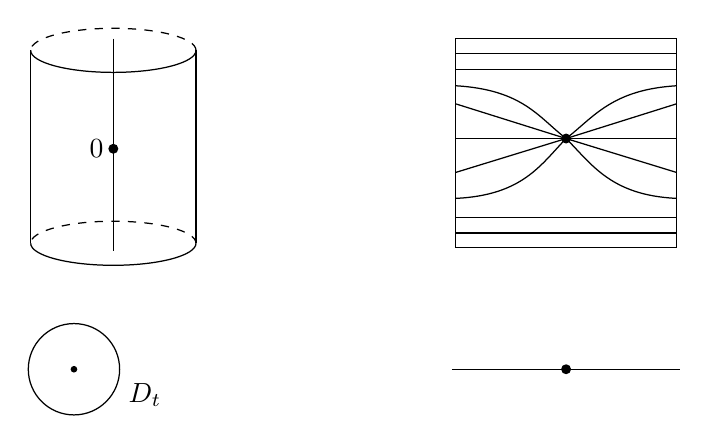
\begin{tikzpicture}[x=1cm,y=1cm,line width=.45pt]
  \draw (-4.2,2.6) arc[start angle=180,end angle=360,x radius=1.05,y radius=.28];
  \draw[dashed] (-2.1,2.6) arc[start angle=0,end angle=180,x radius=1.05,y radius=.28];
  \draw (-4.2,2.6)--(-4.2,.15);
  \draw (-2.1,2.6)--(-2.1,.15);
  \draw (-4.2,.15) arc[start angle=180,end angle=360,x radius=1.05,y radius=.28];
  \draw[dashed] (-2.1,.15) arc[start angle=0,end angle=180,x radius=1.05,y radius=.28];
  \draw (-3.15,2.75)--(-3.15,.05);
  \fill (-3.15,1.35) circle (1.8pt);
  \node[left] at (-3.15,1.35) {$0$};
  \draw (-3.65,-1.45) circle (.58);
  \fill (-3.65,-1.45) circle (1.2pt);
  \node[right] at (-3.08,-1.78) {$D_t$};
  \draw (1.2,.1) rectangle (4.0,2.75);
  \foreach \yy in {.28,.48,2.36,2.56}{\draw (1.2,\yy)--(4.0,\yy);}
  \draw (1.2,2.15) .. controls (2.05,2.10) and (2.25,1.75) .. (2.60,1.48)
                    .. controls (2.95,1.75) and (3.18,2.10) .. (4.0,2.15);
  \draw (1.2,.72) .. controls (2.05,.76) and (2.28,1.15) .. (2.60,1.48)
                   .. controls (2.93,1.15) and (3.17,.76) .. (4.0,.72);
  \draw (1.2,1.92)--(2.60,1.48)--(4.0,1.92);
  \draw (1.2,1.05)--(2.60,1.48)--(4.0,1.05);
  \draw (1.2,1.48)--(4.0,1.48);
  \fill (2.60,1.48) circle (1.8pt);
  \draw (1.15,-1.45)--(4.05,-1.45);
  \fill (2.60,-1.45) circle (1.8pt);
\end{tikzpicture}
\end{center}

Sea $B^+\subset B_{t_0,d_1}$ el conjunto de los puntos $x$ tales que
\[
|f(x)|^2\leq\tau(\delta(x)).
\]
Sea $\varphi_n$ una sucesión de funciones $C^\infty$ de
$[0,t_0]$ en $(0,d_1]$ tal que, para una sucesión
$t_0>r_1>r_2>\cdots$ que tiende a $0$,

\begin{enumerate}[label=(\alph*)]
\item para $|t|^2\geq r_i$, $\varphi_i$ es la función inversa de
  $\tau$;
\item para $|t|^2<r_i$ y $j>i$, se tiene
  $\varphi_j(t)<\varphi_i(t)$.
\end{enumerate}

\begin{center}
\begin{tikzpicture}[x=1cm,y=1cm,>=Latex,line width=.5pt]
  \draw[->] (0,0)--(4.5,0) node[right] {$t$};
  \draw[->] (0,0)--(0,3.4) node[above] {$d$};
  \draw (0,3.0)--(3.05,3.0)--(3.05,0);
  \node[left] at (0,3.0) {$d_1$};
  \node[below] at (3.05,0) {$t_0$};
  \draw (0,0) .. controls (.35,1.05) and (1.35,2.15) .. (3.05,2.45);
  \node[right] at (3.05,2.45) {$t=\tau(d)$};
  \draw (0,1.45) .. controls (.45,1.42) and (.80,1.40) .. (1.18,1.68)
        .. controls (1.45,1.88) and (1.68,2.00) .. (1.92,2.10);
  \node at (.55,1.72) {$\varphi_0$};
  \draw (0,.58) .. controls (.23,.56) and (.35,.65) .. (.50,.90)
        .. controls (.67,1.18) and (.84,1.40) .. (1.18,1.68);
\end{tikzpicture}
\end{center}

El espacio $B^+-\{0\}$ es la unión de los fibrados $B_i^+$ sobre
$D_t$ definidos por
\[
\delta(x)\geq\varphi_i(|f(x)|^2).
\]
Un argumento estándar, que utiliza el hecho de que $\delta$ no tiene
puntos críticos sobre las fibras de $B^+-\{0\}\to D_t$, muestra que
existe un difeomorfismo $\alpha_i:B_i^+\to B_{i+1}^+$, compatible con
la proyección sobre $D_t$ e igual a la identidad fuera de un pequeño
entorno del subespacio

\pageoriginale

\[
\delta(x)=\varphi_i(|f(x)|^2),
\qquad |f(x)|^2\leq r_i,
\]
de $B_i^+$. Componiendo los $\alpha_i$ y pasando al límite, se obtiene
un difeomorfismo
\[
\alpha:B_0^+-\{x\mid f(x)=0,\ \delta(x)=\varphi_0(0)\}
\xrightarrow{\ \sim\ }B^+-\{0\}.
\]
Transportemos mediante $\alpha$ una trivialización del fibrado $B_0^+$
sobre $D_t$ para obtener una conexión integrable $\nabla'$ sobre
$B^+-\{0\}$. Se puede entonces:

\begin{enumerate}[label=(\alph*)]
\item prolongar la restricción de esta conexión a
  $f^{-1}(S_{|y|})\cap B^+$ en una conexión sobre
  $f^{-1}(S_{|y|})/S_{|y|}$; esta prolongación proporciona $T_1$;
\item prolongar a $B_{t_0,d_1}$ el levantamiento, suministrado por
  $\nabla'$ sobre $B^+-\{0\}$, del campo de vectores radial sobre $D_t$.
\end{enumerate}

Existe entonces una única conexión integrable $\nabla$ sobre
$B_{t_0,d_1}$ que prolonga $\nabla'$, (a) y (b), y un único
difeomorfismo horizontal de $B_{t_0,d_1}-\{0\}$ sobre $W-\{0\}$ que
es la identidad sobre $f^{-1}(y)$. Este es el difeomorfismo buscado.

\subsubsection*{3.1.6. Una generalización.}
La exposición precedente se generaliza al caso en que $f:X\to D$ es
un morfismo tal que $0\in X$ es un punto no liso aislado \underline{en}
$X_0$. Tras restringir $X$ y $D$, el lugar no liso de $f$ es entonces
finito sobre $D$. La variedad de ciclos evanescentes $V$ tiene un
conjunto finito $\Sigma$ de puntos críticos; $V-\Sigma$ es una variedad
diferenciable con borde (su borde es compacto, aunque la variedad no lo
sea). La transformación de monodromía $T$ es la identidad en el borde y
estabiliza $\Sigma$. Por último, la Proposición 3.1.5 sigue siendo
válida: el homeomorfismo fibrado $\Psi$ es un difeomorfismo fuera del
lugar crítico, que lleva a la parte de $W$ procedente de $\Sigma$.

\subsubsection*{3.1.7.}
La Proposición 3.1.5 permite utilizar los cálculos de 1.4. Se obtiene:

\begin{enumerate}[label=(\Alph*)]
\item Los grupos de ciclos evanescentes $(R^i\Phi(\Lambda))_0$ son los
  grupos de cohomología reducida, con coeficientes en $\Lambda$, de la
  variedad de ciclos evanescentes $V$.
\item Los grupos $H^i_{\{0\}}(X_0,R\Psi(\Lambda))$ son los grupos de
  cohomología con soporte propio de $V^\circ$, con coeficientes en
  $\Lambda$.
\item La variación

  \pageoriginale

  \[
  \operatorname{Var}:\widetilde H^i(V,\Lambda)
  \longrightarrow H_c^i(V^\circ,\Lambda)
  =H^i(V\bmod\partial V,\Lambda)
  \]
  es la variación clásica definida por el automorfismo $T$ de $V$,
  que es la identidad sobre $\partial V$.
\end{enumerate}

\subsubsection*{3.1.8.}
Las afirmaciones (A), (B) y (C) son, de hecho, más elementales que la
Proposición 3.1.5. Damos una demostración-construcción directa, que evita
comprobar que los isomorfismos de (A) y (B) son independientes de las
elecciones hechas en la construcción de 3.1.5.

Sean $d\leq r$ y $t\leq\tau(d)$, y sea $B$ la caja abierta
\[
B=\{x\mid\delta(x)<d\ \text{y}\ |f(x)|^2<t\}.
\]
Sea $\widetilde D^*$ un recubrimiento universal de $D^*$, y consideremos
el diagrama
\begin{equation}\tag{3.1.8.1}
\begin{tikzcd}[column sep=large,row sep=large]
\{0\} \arrow[r,hook,"\bar\imath"] \arrow[d,equal]
  & \widetilde D_t \arrow[d,"p"]
  & \widetilde D_t^* \arrow[l,hook',"\bar\jmath"'] \arrow[d,"p'"] \\
\{0\} \arrow[r,hook,"i"]
  & D_t
  & D_t^* \arrow[l,hook',"j"']
\end{tikzcd}
\end{equation}
obtenido de (1.2.7.2) por restricción a $D_t$. Sea
\begin{equation}\tag{3.1.8.2}
\begin{tikzcd}[column sep=large,row sep=large]
B_0 \arrow[r,hook,"\bar\imath"] \arrow[d,equal]
  & \overline B \arrow[d,"p"]
  & \overline B^* \arrow[l,hook',"\bar\jmath"'] \arrow[d,"p'"] \\
B_0 \arrow[r,hook,"i"]
  & B
  & B^* \arrow[l,hook',"j"']
\end{tikzcd}
\end{equation}
la imagen inversa de $f:B\to D$ sobre (3.1.8.1). Seguimos denotando
por $f$ la proyección de (3.1.8.2) sobre (3.1.8.1).

\medskip
\noindent\textup{(A)}
Por definición, $R^i\Psi_\eta(\Lambda)_0$ es el límite inductivo,
cuando $U$ recorre los entornos de $0$ en $X$, de los grupos de
cohomología
\[
H^i(U\times_D\widetilde D^*,\Lambda).
\]
Hagamos recorrer a $U$ el sistema fundamental de entornos de $0$
formado por las cajas $B$ anteriores. El producto fibrado
$U\times_D\widetilde D^*=\overline B^*$ es un fibrado de fibra
$V^\circ$ sobre el espacio contráctil $\widetilde D_t^*$. El sistema
inductivo de los grupos $H^i(\overline B^*,\Lambda)$ es, por tanto,
constante, con valor
\[
H^i(V^\circ,\Lambda)=H^i(V,\Lambda).
\]

\pageoriginale

Los isomorfismos resultantes
\begin{equation}\tag{3.1.8.3}
R^i\Psi_\eta(\Lambda)_0\simeq H^i(V,\Lambda)
\end{equation}
pueden precisarse en el isomorfismo compuesto siguiente (cf. (B)):
\begin{equation}\tag{3.1.8.4}
\begin{tikzcd}[column sep=small,row sep=large,cells={nodes={font=\small}}]
R\Psi_\eta(\Lambda)_0
  & R\Gamma(B_0,R\Psi_\eta(\Lambda)) \arrow[l,"\sim"']
  & (Rf_*R\bar\jmath_*\Lambda)_0 \arrow[l,"\sim"']
  & R\Gamma(\widetilde D_t,Rf_*R\bar\jmath_*\Lambda)
      \arrow[l,"\sim"'] \arrow[d,equal] \\
{}
  & R\Gamma(V,\Lambda) \arrow[r,"\sim"]
  & R\Gamma(V^\circ,\Lambda)
  & R\Gamma(\overline B^*,\Lambda) \arrow[l,"\sim"']
\end{tikzcd}
\end{equation}
El complejo $R\Phi(\Lambda)_0$ se define mediante el triángulo distinguido
\[
\Lambda\longrightarrow(R\Psi_\eta\Lambda)_0
\longrightarrow R\Phi(\Lambda)_0\longrightarrow{}.
\]
En consecuencia, los grupos $R^i\Phi(\Lambda)_0$ son los grupos de
cohomología reducida de $V$.

\medskip
\noindent\textup{(B)}
Sea $\mathfrak F$ la familia de cerrados de $\overline B^*$ cuya
adherencia en $\overline B$ es propia sobre $\widetilde D$. Las flechas
del diagrama siguiente son isomorfismos:
\begin{equation}\tag{3.1.8.5}
\begin{tikzcd}[column sep=small,row sep=large,cells={nodes={font=\small}}]
R\Gamma_{\{0\}}(R\Psi_\eta(\Lambda))
  \arrow[r,"\sim","\text{\textcircled{1}}"']
  & R\Gamma_c(B_0,R\Psi_\eta(\Lambda))
  & (Rf_!R\bar\jmath_*\Lambda)_0
      \arrow[l,"\sim"',"\text{\textcircled{2}}"] \\
R\Gamma_c(V^\circ,\Lambda)
  & R\Gamma_{\mathfrak F}(\overline B^*,\Lambda)
      \arrow[l,"\sim"',"\text{\textcircled{5}}"]
      \arrow[r,equal,"\text{\textcircled{4}}"']
  & R\Gamma(\widetilde D_t,Rf_!R\bar\jmath_*\Lambda)
      \arrow[u,"\text{\textcircled{3}}","\wr"']
\end{tikzcd}
\end{equation}
En efecto, \textcircled{1} es un isomorfismo porque $B_0$ es un cono
(3.1.2) y $R^i\Psi_\eta(\Lambda)$ es constante fuera de $0$;
\textcircled{2}, por el teorema de cambio de base propio;
\textcircled{3}, porque $Rf_!R\bar\jmath_*\Lambda$ es constante fuera de
$0$; \textcircled{4} es la versión en categorías derivadas de la
sucesión espectral de un funtor compuesto; y \textcircled{5}, porque
$\widetilde D^*$ es contráctil.

El isomorfismo (3.1.8.5) proporciona los isomorfismos buscados

\pageoriginale

\begin{equation}\tag{3.1.8.6}
R^i\Gamma_{\{0\}}(R\Psi_\eta(\Lambda))
\simeq H_c^i(V^\circ,\Lambda).
\end{equation}
Comprobaremos (C) en 3.1.10.

\subsubsection*{3.1.9.}
Cf. [3]. Sea $X$ un espacio topológico, sea $i:Y\hookrightarrow X$ un
cerrado, sea $T$ un automorfismo de $X$ que induce la identidad sobre
$Y$, y sea $\Lambda$ un grupo abeliano. Para definir la variación
$\operatorname{Var}$, elijamos una resolución $T$-equivariante
$\Lambda_X^*$ de $\Lambda$ sobre $X$, una resolución $\Lambda_Y^*$ del
haz constante $\Lambda$ sobre $Y$, sobre la cual $T$ actúa trivialmente
por convención, y un morfismo equivariante
\[
\varphi:\Lambda_X^*\longrightarrow i_*\Lambda_Y^*
\]
que resuelve el morfismo evidente
$\varphi_0:\Lambda_X\to i_*\Lambda_Y$. Supongamos que los haces
$\Lambda_X^i$ y $\Lambda_Y^i$ son acíclicos para los funtores que se
consideran. Pasando a las secciones globales, se obtiene
\[
\Gamma(\varphi):\Gamma(\Lambda_X^*)
\longrightarrow\Gamma(\Lambda_Y^*).
\]
Por simplicidad, supongamos que todo $\Gamma(\varphi)^i$ es sobreyectivo;
si no, hágase sobreyectivo adjuntando el cono de
$\Gamma(\Lambda_Y^*)$ a $\Gamma(\Lambda_X^*)$. Pongamos
\[
R\Gamma(X\bmod Y,\Lambda)=\operatorname{Ker}(\Gamma(\varphi)).
\]
Bajo hipótesis razonables, si $\mathfrak F$ es la familia de cerrados de
$X$ disjuntos de $Y$, existe un cuasi-isomorfismo
\[
\Gamma_{\mathfrak F}(X-Y,\Lambda_X^*)
\xrightarrow{\ \sim\ }R\Gamma(X\bmod Y,\Lambda).
\]
El endomorfismo $T-1$ de $\Gamma(\Lambda_X^*)$, donde $T$ actúa por
transporte de estructura, es nulo sobre $\Lambda$ (las constantes) y
se factoriza por $\operatorname{Ker}(\Gamma(\varphi))$. Por tanto, en la
categoría derivada y bajo las mismas hipótesis, proporciona un morfismo
de variación
\[
\operatorname{Var}:R\widetilde\Gamma(X,\Lambda)
\longrightarrow R\Gamma_{\mathfrak F}(X-Y,\Lambda).
\]

\pageoriginale

Sin estas hipótesis, se obtiene en su lugar
\[
\operatorname{Var}:R\widetilde\Gamma(X,\Lambda)
\longrightarrow R\Gamma(X\bmod Y,\Lambda).
\]

Esta descripción se simplifica cuando $T$ es la identidad en un entorno
de $Y$ y actúa como la identidad sobre $\Lambda_X^*$ en ese entorno. El
endomorfismo $T-1$ de $\Gamma(\Lambda_X^*)$ se factoriza entonces por
$\Gamma_{\mathfrak F}(\Lambda_X^*)$ y proporciona la variación.

\subsubsection*{Proposición 3.1.10.}
Bajo los isomorfismos de 3.1.8(A),(B), la variación
\[
(R\Phi_\eta(\Lambda))_0
\longrightarrow R\Gamma_{\{0\}}(R\Psi_\eta(\Lambda))
\]
es igual a la variación de 3.1.9 definida por el automorfismo $T$ de
$V$, que es la identidad sobre $\partial V$.

Se invita al lector a hacer un pequeño dibujo en lugar de leer la
demostración. Sea ${}_fB$ la caja cerrada de 3.1.2 y sea
${}_fC\subset{}_fB$ un collar a lo largo del borde; así,
${}_fC\simeq\partial_fB\times[0,1]$ como fibrado sobre $D_t$, mediante
un isomorfismo que lleva $\partial_fB\times\{1\}$ idénticamente sobre
$\partial_fB$. Sea
\[
{}_f\alpha:{}_fC\xrightarrow{\ \sim\ }
(\partial V\times[0,1])\times D_t
\]
una trivialización del fibrado ${}_fC$ sobre $D_t$ cuya fibra en
$y\in D_t$ induce la identidad
\[
\partial V=\partial(f^{-1}(y))
\xrightarrow{\ \sim\ }\partial V\times\{1\}.
\]
Pongamos $C={}_fC\cap B$ y sea
\[
\alpha:C\xrightarrow{\ \sim\ }
(\partial V\times[0,1))\times D_t
\]
el isomorfismo inducido por ${}_f\alpha$. Conservamos la notación de
(3.1.8.2).

Sea $R$ la relación de equivalencia sobre $\overline B$ definida por
$xRy$ si $x=y$, o si $p(x),p(y)\in C$ y $\alpha(p(x))$,
$\alpha(p(y))$ tienen la misma imagen en $\partial V\times[0,1)$.
Pongamos
\[
{}_1\overline B=\overline B/R,
\qquad
{}_1\overline B^*=\overline B^*/R,
\qquad
{}_1\overline C^*=p^{-1}(C)/R.
\]
Hay un diagrama conmutativo

\pageoriginale

\[
\begin{tikzcd}[column sep=large,row sep=large]
B_0 \arrow[r,hook,"\bar\imath"] \arrow[d,equal]
  & \overline B \arrow[d,"q"]
  & \overline B^* \arrow[l,hook',"\bar\jmath"'] \arrow[d,"q'"] \\
B_0 \arrow[r,hook,"\bar\imath"]
  & {}_1\overline B
  & {}_1\overline B^* \arrow[l,hook',"{}_1\bar\jmath"']
\end{tikzcd}
\]
Sea $\Lambda^*$ una resolución $\pi_1(D^*)$-equivariante de $\Lambda$
por haces acíclicos sobre $\overline B^*$. Por definición, la variación
se calcula a partir del morfismo de complejos
\[
\Lambda[0]\longrightarrow
\bar\imath^*\bar\jmath_*(\Lambda^*).
\]
Como $\Lambda\xrightarrow{\sim}Rq_*\Lambda$ y
$\Lambda\xrightarrow{\sim}Rq'_*\Lambda$, puede calcularse igualmente
mediante una resolución equivariante de $\Lambda$ sobre
${}_1\overline B^*$ y el morfismo
\[
\Lambda[0]\longrightarrow
\bar\imath^*{}_1\bar\jmath_*(\Lambda).
\]
Bajo (A) y (B), la variación se identifica así con el morfismo compuesto
\begin{equation}\tag{3.1.10.1}
\begin{tikzcd}[column sep=small,row sep=large,cells={nodes={font=\small}}]
R\Gamma(V,\Lambda) \arrow[r,"\sim"]
  & R\Gamma(V^\circ,\Lambda)
  & R\Gamma({}_1\overline B^*,\Lambda)
      \arrow[l,"\sim"',"\text{\textcircled{1}}"]
      \arrow[d,"\operatorname{Var}"] \\
{}
  & R\Gamma_c(V^\circ,\Lambda)
  & R\Gamma({}_1\overline B^*\bmod{}_1\overline C^*,\Lambda)
      \arrow[l,"\sim"',"\text{\textcircled{2}}"]
\end{tikzcd}
\end{equation}
donde \textcircled{1} y \textcircled{2} son inducidos por la inclusión
de $V^\circ$ en ${}_1\overline B^*$, y donde $\operatorname{Var}$ es la
variación de 3.1.9 para ${}_1\overline B^*$ y la acción del generador
positivo de $\pi_1(D^*)$. Este grupo actúa sobre ${}_1\overline B^*$ por
la acción descrita en 1.1.5 y actúa trivialmente sobre
${}_1\overline C^*$.

Elijamos una conexión $\nabla$ sobre $B^*/D^*$ compatible con la
trivialización de $C$. Esta conexión trivializa $\overline B^*$ y,
pasando al cociente, define una aplicación
$u:{}_1\overline B^*\to V$. Para $T$ definida como en 3.1.3, el diagrama

\pageoriginale

\[
\begin{tikzcd}[column sep=large,row sep=large]
{}_1\overline B^* \arrow[r,"u"] \arrow[d,"T"']
  & V \arrow[d,"T"] \\
{}_1\overline B^* \arrow[r,"u"]
  & V
\end{tikzcd}
\]
es conmutativo. La aplicación $u$ induce isomorfismos en cohomología, de
modo que la Proposición 3.1.10 resulta de (3.1.10.1) y de la funtorialidad
de la variación.

La Proposición 3.1.10 tiene por objeto justificar un cálculo explícito
que se efectuará más adelante y en el cual, como aquí, $T$ es la
identidad en un entorno de $\partial V$. Se tomará una clase de
cohomología $c$ representada por una corriente $C$ y se utilizará el
hecho de que $\operatorname{Var}(c)$ está representada por la corriente
$TC-C$, de soporte compacto en $V^\circ$.

\subsubsection*{3.1.11.}
En la práctica, $T$ se calcula a menudo en dos etapas.

\begin{enumerate}[label=(\alph*)]
\item Fijemos $t$ y $d$ tales que $t\leq\tau(d)$, elijamos
  $y\in D_t^*$ y elijamos una conexión $\nabla$ sobre
  $f^{-1}(S_{|y|})\cap B_{t,d}$. Esta conexión define un
  difeomorfismo $T_0$ de
  \[
  V_0=f^{-1}(y)\cap B_{t,d}
  \]
  sobre sí mismo, que no tiene por qué ser la identidad en el borde.
\item Elijamos una trivialización de $\partial B_{t,d}$ sobre $D_t$.
  La integración de $\nabla$ proporciona un difeomorfismo
  $\varphi(\theta)$ de $\partial V$ sobre
  \[
  f^{-1}(e^{2\pi i\theta}y)\cap\partial B_{t,d},
  \]
  que se identifica con $\partial V$ mediante la trivialización. Para
  $0\leq\theta\leq1$, $\varphi(\theta)$ es un camino en
  $\operatorname{Diff}(\partial V)$ que une la identidad con
  $\partial T_0$.
\end{enumerate}

El par resultante $(T_0,\varphi)$ depende de las elecciones arbitrarias
realizadas. Como el espacio de estas elecciones es contráctil, es
independiente de ellas salvo homotopía. Para una transformación $T$ del
tipo considerado en 3.1.3, $(T,\text{camino constante})$ es un par del
tipo considerado aquí.

\subsubsection*{3.1.12.}
La aplicación
\[
\operatorname{Diff}(V)\longrightarrow\operatorname{Diff}(\partial V)
\]
es una fibración. En consecuencia, la asignación
$T\mapsto(T,\text{camino constante})$ induce una biyección entre:

\begin{enumerate}[label=\alph*)]
\item los difeomorfismos $T:V\to V$ tales que
  $\partial T=\operatorname{id}$, salvo isotopía; y

  \pageoriginale

\item los pares $(T_0,\varphi)$, donde
  $T_0:V\xrightarrow{\sim}V$ y $\varphi$ es una clase de homotopía
  de caminos desde $\operatorname{id}$ hasta $\partial T_0$, salvo
  isotopía.
\end{enumerate}

Un par $(T_0,\varphi)$ calculado mediante 3.1.11(a),(b) determina, por
tanto, $T$. Concretamente, se calcula $T$ a partir de
$(T_0,\varphi)$ como sigue.

\medskip
\noindent\textup{($\alpha$)} Elijamos una inmersión de collar
\[
[0,1]\times\partial V\xhookrightarrow{\ \alpha\ }V,
\qquad \alpha(1,x)=x,
\]
y un representante
$\varphi:[0,1]\to\operatorname{Diff}(\partial V)$ tal que su
prolongación por $\operatorname{id}$ para parámetros negativos sea de
clase $C^\infty$. Sobre el collar, pongamos
\[
\beta(x)=\operatorname{pr}_1\alpha^{-1}(x).
\]
Así, $\beta$ no tiene punto crítico, toma valores en $[0,1]$ y vale
$1$ sobre $\partial V$.

\medskip
\noindent\textup{($\beta$)} Tomemos $T=T_0$ fuera del collar y, sobre
el collar, pongamos
\[
T(x)=T_0\bigl(\varphi(\beta(x))^{-1}(x)\bigr).
\]

\subsubsection*{3.1.13.}
He aquí una variante de 3.1.11(b) para calcular la clase de homotopía
del camino $\varphi$. Sobre cada rayo $\arg(z)=\theta$, elijamos una
trivialización del fibrado $\partial B_{t,d}$ que varíe continuamente
con $\theta$. Utilicemos la trivialización sobre el rayo que pasa por
$y$ para identificar
\[
(\partial V)_0=f^{-1}(0)\cap\partial B_{t,d}
\]
con $\partial V$. Sea
\[
\Psi_\theta:V\longrightarrow
f^{-1}(e^{i\theta}y)\cap B_{t,d}
\]
la aplicación obtenida integrando $\nabla$. Transportando
$\partial\Psi_\theta$ a lo largo de los rayos, se obtiene un
difeomorfismo de $(\partial V)_0$, y por tanto de $\partial V$, sobre
sí misma. Este es $\varphi(\theta)$.

\subsection*{3.2. La fórmula de Picard--Lefschetz (caso trascendente)}

\subsubsection*{3.2.1.}
Explicitaremos los resultados de 3.1 para la aplicación
\[
f=\sum_{i=1}^{n+1}z_i^2:\mathbb C^{n+1}\longrightarrow\mathbb C.
\]
Para $\delta$, tomemos la función $\sum |z_i|^2$, y tomemos la caja
$B=B_{a,b}$ definida por
\[
\left|\sum z_i^2\right|\leq a^2,
\qquad
\sum |z_i|^2\leq b^2,
\]
con $0<a<b$. Solo para simplificar la notación se toma una caja

\pageoriginale

cerrada en lugar de una caja como en 3.1.2.

\subsubsection*{3.2.2.}
La variedad de ciclos evanescentes $V$ tiene ecuaciones
\begin{equation}\tag{3.2.2.1}
\begin{array}{rcl}
\displaystyle\sum z_i^2&=&a^2,\\
\displaystyle\sum |z_i|^2&\leq&b^2.
\end{array}
\end{equation}
Escribamos $z=(z_i)$ en términos de sus partes real e imaginaria,
$z=x+iy$. Las ecuaciones precedentes se convierten en
\begin{equation}\tag{3.2.2.2}
\begin{array}{rcl}
x^2-y^2&=&a^2,\\
x\mathbin{\cdot}y&=&0
  \qquad\bigl(\text{es decir, }x\perp y\text{ en }
  \mathbb R^{\sisi{n}{n+1}}\bigr),\\
x^2+y^2&\leq&b^2.
\end{array}
\end{equation}
Introduzcamos sobre $V$ el nuevo sistema de coordenadas
\[
X=\frac{x}{|x|},
\qquad
Y=y\left(\frac{b^2-a^2}{2}\right)^{-1/2}.
\]
Entonces $x=X(a^2+y^2)^{1/2}$, y (3.2.2.2) se transforma en
\begin{equation}\tag{3.2.2.3}
\begin{array}{rcl}
X^2&=&1,\\
X\mathbin{\cdot}Y&=&0,\\
Y^2&\leq&1.
\end{array}
\end{equation}
Esto identifica $V$ con el fibrado de bolas tangentes de la esfera
$S^n$.

\subsubsection*{3.2.3.}
La aplicación
\[
\theta\longmapsto \exp(2\pi i\theta)a
\]
identifica $\mathbb R$ con el recubrimiento universal del círculo
$S_a$ de $\mathbb C$ de radio $a$ y centro $0$. La imagen inversa sobre
$\mathbb R$ del fibrado $B$ es isomorfa a $\mathbb R\times V$. La
trivializamos mediante el isomorfismo
\[
v\longmapsto \exp(\pi i\theta)v
\]
de $V$ sobre la fibra de $B$ situada encima de
$\exp(2\pi i\theta)a$. Sea $T_0$ la aplicación proporcionada por esta
trivialización como en 3.1.11. En las coordenadas (3.2.2.3),
\[
T_0(X,Y)=(-X,-Y).
\]

\subsubsection*{3.2.4.}
El fibrado sobre el disco $D_a$ de radio $a$ que forma el borde del
``fibrado'' $B$ tiene ecuaciones
\[
\sum |z_i|^2=b^2,
\qquad
f(z)\in D_a,
\]

\pageoriginale

siendo $f$ la proyección sobre el disco. Nos proponemos describir una
trivialización de la imagen inversa de este fibrado sobre cada uno de
los rayos
\[
e^{2\pi i\theta}\mathbb R^+\cap D_a.
\]

Sobre el rayo $\mathbb R^+\cap D_a$, tomemos el isomorfismo con
$(\mathbb R^+\cap D_a)\times\partial V$ dado, en las coordenadas
(3.2.2.3) sobre $\partial V$, por
\[
z=x+iy\longmapsto(f(z),X,Y)
  =\left(f(z),\frac{x}{|x|},\frac{y}{|y|}\right).
\]
Sobre $(e^{2\pi i\theta}\mathbb R^+)\cap D_a$, utilicemos la imagen de
esta trivialización por la multiplicación por $e^{\pi i\theta}$.
Apliquemos 3.1.13 y utilicemos sobre $\partial V$ las coordenadas $(X,Y)$
que satisfacen
\begin{equation}\tag{3.2.4.1}
X^2=Y^2=1,
\qquad
X\mathbin{\cdot}Y=0.
\end{equation}
Si $\varphi(\theta)$ lleva $(X,Y)$ a $(X_\theta,Y_\theta)$, se obtiene
\begin{equation}\tag{3.2.4.2}
X_\theta+iY_\theta
=e^{\pi i\theta}(X+iY)
\qquad(0\leq\theta\leq1).
\end{equation}

\subsubsection*{3.2.5.}
En resumen, la variedad de ciclos evanescentes $V$ es el fibrado de
bolas tangentes de $S^n$. La transformación de monodromía está
representada por $(T_0,\varphi)$, donde $T_0$ es la diferencial de la
aplicación antipodal y $\varphi$ es el camino siguiente desde
$\operatorname{Id}$ hasta $\partial T_0$: bajo $\varphi(\theta)$,
cada vector tangente unitario es transportado paralelamente a lo largo
de la geodésica que determina una distancia $+\pi\theta$ (el signo
positivo significa ``en el sentido en que apunta el vector''). Para
$\theta=1$, se alcanza el vector antipodal.

Por 3.1.13, esto da la descripción siguiente de $T$. Sea
$\varphi:[0,1]\to[0,1]$ una aplicación $C^\infty$ que vale $0$ en un
entorno de $0$ y $1$ en un entorno de $1$. La aplicación $T$ desplaza
$u$, a lo largo de la geodésica que $u$ determina, una distancia
\[
-\pi\bigl(1-\varphi(|u|)\bigr).
\]
En un entorno de $|u|=1$ es la identidad; en un entorno de $|u|=0$ es
la aplicación antipodal.

\subsubsection*{3.2.7.}
Sea $W$ una variedad diferenciable de dimensión $\sisi{x}{d}$, y sea
\[
p:T(W)\longrightarrow W
\]
su fibrado tangente, considerado como variedad.

\pageoriginale

Si $(x_1,\ldots,x_{\sisi{n}{d}})$ es un sistema de coordenadas locales
sobre $W$, entonces
\[
(x_1,\ldots,x_d,dx_1,\ldots,dx_d)
\]
es un sistema de coordenadas locales sobre $T(W)$. Sea $\varepsilon'$
la orientación de $T(W)$ definida por este sistema de coordenadas. No
depende de la elección de los $x_i$ y, por tanto, está definida
globalmente.

Supongamos que $W$ es orientable. La subvariedad $W\subset T(W)$ (la
sección cero), dotada de una orientación (respectivamente, de una
orientación de su fibrado normal), define un elemento $w$ de
$H_d(T(W))$ (respectivamente, de $H_c^d(T(W))$). La autointersección
de $W\subset T(W)$ es la característica de Euler--Poincaré:
\[
\int w\wedge w=\chi(W)
\]
para la orientación $\varepsilon'$.

Para la variedad de ciclos evanescentes $V$, su estructura compleja
define una orientación $\varepsilon$. Está relacionada con la orientación
$\varepsilon'$ del fibrado tangente de $S^n$ por
\[
\varepsilon=(-1)^{\frac{n(n-1)}2}\varepsilon'.
\]

\subsubsection*{3.2.8.}
El \underline{ciclo evanescente} $\delta$ está bien definido salvo signo.
Para $n\ne0$, es el elemento de $H_c^n(V^\circ)$ definido por la
subvariedad $S^n\subset V^\circ$. Para $n=0$, el espacio $V$ consta de
dos puntos, y $\delta$ es su diferencia. Con la orientación compleja de
$V$, 3.2.7 da
\begin{equation}\tag{3.2.8.1}
(\delta,\delta)
=(-1)^{\frac{n(n-1)}2}\bigl(1+(-1)^n\bigr).
\end{equation}

\subsubsection*{3.2.9.}
Pongamos
\[
\widetilde H_c^i(V^\circ)
=\operatorname{Ker}\!\left(
H_c^i(V^\circ)\xrightarrow{\ \operatorname{Tr}\ }\mathbb Z
\right);
\]
esto es $H_c^i(V^\circ)$ para $i\ne2n$. Entonces
\[
\begin{aligned}
\widetilde H_c^i(V^\circ)&=0 &&\text{para }i\ne n,\\
\widetilde H_c^n(V^\circ)&=\mathbb Z,
  &&\text{engendrado por }\delta.
\end{aligned}
\]
Dualemente,
\[
\begin{aligned}
\widetilde H^i(V)&=0 &&\text{para }i\ne n,\\
\widetilde H^n(V)&\xrightarrow[\sim]{\ (\,\cdot\,,\delta)\ }\mathbb Z.
\end{aligned}
\]

\pageoriginale

Para $n\ne0$, la imagen de $\delta\in H_c^n(V^\circ)$ en $H^n(V)$
es nula cuando $n$ es impar y divisible por dos (y no más) cuando $n$
es par.

\subsubsection*{3.2.10.}
Calculemos la variación
\[
\operatorname{Var}:\widetilde H^n(V)
\longrightarrow H_c^n(V^\circ).
\]
Utilicemos primero la orientación $\varepsilon'$ y supongamos que
$n\ne0$. Sea $\alpha$ una orientación del fibrado tangente de $S^n$, y
sea $\delta\in H_c^n(V^\circ)$ definida por $S^n\subset V^\circ$ junto
con la orientación $\alpha$ de su fibrado normal. El cociclo
$\delta'\in H^n(V)$ tal que $(\delta',\delta)=1$ está representado por
una fibra de la fibración de $V^\circ$ sobre $S^n$. El fibrado normal de
esta fibra es el fibrado constante de valor el espacio tangente en un
punto de $S^n$, y está dotado de la orientación $\alpha$.

Esta afirmación es independiente de la convención de signo elegida para
definir la aplicación
\[
(\text{subvariedad + orientación de su fibrado normal})
\longrightarrow\text{cohomología}.
\]
En efecto, cambiar la convención cambia $\delta$ por $-\delta$ y
$\delta'$ por $-\delta'$. La afirmación es válida cuando
\[
\operatorname{Tr}:H_c^{2n}(V,\mathbb R)\longrightarrow\mathbb R
\]
se define como sigue:
\begin{description}[leftmargin=2.8em,labelsep=.5em]
\item[\textup{($\alpha$)}] puesto que $\Omega_V^*$ es una resolución
  fina de $\underline{\mathbb R}$, $\Gamma_c(\Omega_V^*)$ representa
  $R\Gamma_c(V,\mathbb R)$, de donde resulta un isomorfismo
  \[
  H^i\bigl(\Gamma_c(V,\Omega_V^*)\bigr)
  \simeq H_c^i(V,\mathbb R)
  \]
  (no se utiliza el coborde iterado);
\item[\textup{($\beta$)}] $\operatorname{Tr}$ es la integración.
\end{description}

La clase $T(\delta')$ coincide con $\delta'$ en un entorno de
$\partial V$, de modo que
$\operatorname{Var}(\delta')=T(\delta')-\delta'$ tiene soporte compacto
en $V^\circ$. Se tiene
\[
T(\delta')-\delta'\sim-\delta,
\qquad\text{y, por tanto,}
\]
\[
\operatorname{Var}(\delta')
=-(\delta',\delta)\,\delta.
\]

He aquí el dibujo para $n=1$. Dibujamos el fibrado tangente de $S^1$
de modo que los vectores que apuntan en la orientación antihoraria
elegida de $S^1$ apunten hacia el exterior.

\pageoriginale

\begin{center}
\begin{tikzpicture}[>=Latex,line width=.45pt,scale=.92]
  \begin{scope}[shift={(-2.8,0)}]
    \draw (0,0) circle (2.15);
    \draw (0,0) circle (1.20);
    \draw (0,0) circle (.43);
    \draw (0,.43)--(0,2.15);
    \draw[->] (-.02,1.88)--(-.48,1.88);
    \draw[->] (-.02,1.13)--(-.48,1.13);
    \node[right] at (.10,1.10) {$\delta'$};
    \draw[->] (-.85,.85)--(-1.16,1.16);
    \draw[->] (-.85,-.85)--(-1.17,-1.17);
    \node[above left] at (-1.02,-.98) {$\delta$};
    \draw[->] (.85,-.85)--(1.17,-1.17);
    \draw[->] (1.43,1.12)--(1.43,1.72)
      node[right] {$2$};
    \draw[->] (1.43,1.12)--(.83,1.12)
      node[below] {$1$};
    \node at (1.03,1.63) {$\varepsilon$};
    \node[below=5pt] at (0,-2.15)
      {$\delta,\ \delta'\ \text{y}\ \varepsilon$};
  \end{scope}
  \begin{scope}[shift={(2.8,0)}]
    \draw (0,0) circle (2.15);
    \draw (0,0) circle (.43);
    \draw (0,.43)--(0,2.15);
    \draw
      (0,2.15)
      .. controls (.02,1.68) and (1.18,1.42) .. (1.28,.30)
      .. controls (1.40,-.72) and (.62,-1.35) .. (-.12,-1.31)
      .. controls (-1.05,-1.27) and (-1.42,-.42) .. (-1.10,.48)
      .. controls (-.83,1.10) and (-.34,1.25) .. (0,1.02);
    \draw[->] (1.08,.78)--(.74,.48);
    \node[below=5pt] at (0,-2.15)
      {$\operatorname{Var}(\delta')$};
  \end{scope}
\end{tikzpicture}
\end{center}

Para la orientación $\varepsilon$, se tiene, por consiguiente,
\[
\operatorname{Var}(x)
=-\frac{\varepsilon}{\varepsilon'}(x,\delta)\,\delta.
\]

\subsubsection*{Teorema 3.2.11.}
\underline{El grupo $\widetilde H_c^n(V^\circ)$ es isomorfo a
$\mathbb Z$, engendrado por el ciclo evanescente $\delta$. El grupo
$\widetilde H^n(V)$ también es isomorfo a $\mathbb Z$ y es dual del
grupo precedente. Todos los demás grupos
$\widetilde H_c^i(V^\circ)$ y $\widetilde H^i(V)$ son nulos.}

\medskip
\noindent\underline{La variación viene dada por}
\[
\operatorname{Var}(x)
=-(-1)^{\frac{n(n-1)}2}(x,\delta)\,\delta,
\qquad\underline{\text{y}}
\]
\[
(\delta,\delta)
=(-1)^{\frac{n(n-1)}2}\bigl(1+(-1)^n\bigr).
\]
Según la clase de congruencia de $n$ módulo $4$, se tiene la tabla
siguiente:
\[
\begin{array}{lcccc}
n\bmod4&0&1&2&3\\[2pt]
(\delta,\delta)&2&0&-2&0\\[2pt]
\operatorname{Var}(x)=\pm(x,\delta)\delta&-&-&+&+\\[2pt]
T(\delta)=(-1)^{n+1}\delta&-\delta&\delta&-\delta&\delta
\end{array}
\]
Como comprobación, se tiene, en efecto,
\[
T(\delta)=\delta+\operatorname{Var}(\delta).
\]

\pageoriginale

\section*{4. Cohomología de De Rham}

\subsubsection*{4.1.}
Sea $D$ un disco analítico complejo, sea $0\in D$, pongamos
$D^*=D-\{0\}$, y sea $\widetilde D^*$ un recubrimiento universal de
$D^*$. Sea $X$ un espacio analítico, sea
$f:X\longrightarrow D$ un morfismo, y consideremos el diagrama de
(1.2.7.1):
\begin{equation}\tag{4.1.1}
\begin{tikzcd}[column sep=large,row sep=large]
X_0 \arrow[r,hook,"\bar i"] \arrow[d,equal]
  & \bar X \arrow[d,"p"']
  & \bar X^* \arrow[l,hook',"\bar j"'] \arrow[d,"p'"'] \\
X_0 \arrow[r,hook,"i"]
  & X
  & X^* \arrow[l,hook',"j"']
\end{tikzcd}
\end{equation}
Supongamos que $X^*=X-X_0$ es no singular (es decir, liso). Su
recubrimiento $\bar X^*$ es, por tanto, liso. Denotemos por
$\Omega_{\bar X^*}^*$ el complejo de De Rham de haces de formas
diferenciales holomorfas sobre $\bar X^*$. Es una resolución del haz
constante $\mathbb C$ (lema de Poincaré holomorfo) y proporciona, por
tanto, un morfismo
\begin{equation}\tag{4.1.2}
\bar j_*\Omega_{\bar X^*}^*
\longrightarrow R\bar j_*\mathbb C
\end{equation}
en $D^+(\bar X,\mathbb C)$.

\subsubsection*{Proposición 4.2.}
\underline{El morfismo (4.1.2) es un isomorfismo.}

Es claro que \sisi{(4.1.1)}{(4.1.2)} es un cuasi-isomorfismo en todo
punto de $\bar X^*\subset\bar X$. Basta, por tanto, mostrar que todo
punto $x\in X_0$ tiene un sistema fundamental de entornos $U$ en
$\bar X$ tales que
\[
H^q\bigl(\bar j^{-1}(U),\Omega^p\bigr)=0
\qquad\text{para }q>0.
\]
Cuando $V$ recorre un sistema fundamental de entornos de $x$ en $X$,
los conjuntos $p^{-1}(V)$ forman un sistema fundamental de entornos de
$x$ en $\bar X$. En particular, se pueden tomar los $p^{-1}(V)$ para
$V$ un entorno de Stein de $x$ en $X$. Si $V$ es de Stein, entonces
$V-X_0$ sigue siendo de Stein (pues $X_0\cap V$ está definido por una
ecuación en $V$), al igual que su recubrimiento
\[
p'^{-1}(V-X_0)=\bar j^{-1}p^{-1}(V).
\]

\pageoriginale

En consecuencia, para todo haz coherente $\mathcal F$ sobre
$\bar X^*$,
\[
H^q\bigl(\bar j^{-1}p^{-1}(V),\mathcal F\bigr)=0
\qquad\text{para }q>0,
\]
lo que demuestra la proposición.

\subsubsection*{Corolario 4.3.}
\underline{El isomorfismo (4.1.2) induce un isomorfismo}
\begin{equation}\tag{4.3.1}
\bar i^*\bar j_*\Omega_{\bar X^*}^*
\xrightarrow{\ \sim\ }R\Psi_\eta(\mathbb C).
\end{equation}

\subsubsection*{Variante 4.4.}
\underline{Sea $V$ un haz localmente constante de espacios vectoriales
complejos de dimensión finita sobre $X^*$ (un sistema local complejo).
El cuasi-isomorfismo}
\[
V\longrightarrow\Omega_{X^*}^*(V)
\]
\underline{del lema de Poincaré induce un cuasi-isomorfismo}
\begin{equation}\tag{4.4.1}
\bar i^*\bar j_*\Omega_{\bar X^*}^*(p'^*V)
\xrightarrow{\ \sim\ }R\Psi_\eta(V).
\end{equation}

Mostraremos que (4.3.1) sigue siendo cierto cuando se reemplaza
$\bar i^*\bar j_*\Omega_{\bar X^*}^*$ por un subcomplejo definido por
condiciones de crecimiento y de monodromía.

\subsubsection*{4.5.}
Sea $f:X^*\longrightarrow D^*$ un espacio topológico sobre $D^*$,
sea $F$ un haz de $f^\circ\mathcal O_{D^*}$-módulos sobre $X^*$, y
sea $\bar F$ su imagen inversa sobre
\[
\bar X^*=X^*\times_{D^*}\widetilde D^*.
\]

Sea $z:D\hookrightarrow\mathbb C$ una inmersión holomorfa tal que
$z(0)=0$. En lo sucesivo siempre podremos restringir $D$; para un disco
suficientemente pequeño, la existencia de $z$ es trivial. Elijamos sobre
$\widetilde D^*$ una función $\log z$ tal que $\exp(\log z)=z$, y
pongamos
\[
z^\alpha=\exp(\alpha\log z)
\qquad(\alpha\in\mathbb C).
\]

El grupo $\pi_1(D^*)$ actúa, por transporte de estructura, sobre
$H^0(\bar X^*,\bar F)$. Un elemento $f\in H^0(\bar X^*,\bar F)$ es de
\underline{determinación finita} si sus transformados bajo
$\pi_1(D^*)$ engendran un espacio vectorial complejo de dimensión finita
$V(\sisi{F}{f})$. Sea $T$ el generador positivo de $\pi_1(D^*)$. La
sección $f$ es de determinación finita si y solo si existe un polinomio
no nulo $P\in\mathbb C[X]$ tal que

\pageoriginale

$P(T)(f)=0$. El polinomio de menor grado con esta propiedad es entonces
a la vez el polinomio minimal y el polinomio característico de $T$
actuando sobre $V(f)$.

Se dice que $f$ es de \underline{determinación finita unipotente} si
existe un $A$ tal que
\[
(T-1)^A f=0.
\]
Sobre el espacio de estas secciones, se define
\[
N=\frac{\log T}{2\pi i}
\]
mediante la suma finita
\[
N(f)=-\frac1{2\pi i}
\sum_{n>0}\frac{(1-T)^n}{n}\,f.
\]
Si $f$ (respectivamente, $g$) es una sección de determinación finita
unipotente en $H^0(D^*,\mathcal O)$ (respectivamente, en
$H^0(\bar X^*,\bar F)$), entonces
\[
N(fg)=N(f)g+fN(g),
\]
pues el logaritmo de un automorfismo es una derivación.

Se dice que $f$ es de
\underline{determinación finita cuasi-unipotente} si existen $A$ y
$B>0$ tales que
\[
(T^B-1)^A f=0.
\]

\subsubsection*{Ejemplos 4.6.}
Para $X=D^*$ y $F=\mathcal O$, se tiene
\[
\bigl(T-\exp(2\pi i\alpha)\bigr)^{k+1}
  \bigl(z^\alpha(\log z)^k\bigr)=0,
\]
\[
N(\log z)=1,
\]
y
\[
N\left(\frac{(\log z)^k}{k!}\right)
=\frac{(\log z)^{k-1}}{(k-1)!},
\qquad
(0\text{ para }k=0).
\]

\subsubsection*{Proposición 4.7.}
\underline{Una sección $f\in H^0(\bar X^*,\bar F)$ es de determinación
finita si y solo si puede escribirse}
\begin{equation}\tag{4.7.1}
f=\sum_{\alpha,k}f_{\alpha,k}\,
z^\alpha\frac{(\log z)^k}{k!},
\end{equation}
\underline{donde $0\leq\operatorname{Re}(\alpha)<1$,
$k\in\mathbb N$, y los
$f_{\alpha,k}\in H^0(X^*,F)$ son casi todos nulos. Para $f$ de
determinación finita, la descomposición (4.7.1) es única.}

\pageoriginale

Por 4.6, toda sección de la forma (4.7.1) es de determinación finita.
Recíprocamente, sea $f$ de determinación finita, con $P(T)(f)=0$.
Escribamos
\[
P(X)=\prod_{\beta\in\mathbb C}(X-\beta)^{n'(\beta)}
=\prod_{0\leq\operatorname{Re}(\alpha)<1}
 \bigl(X-\exp(2\pi i\alpha)\bigr)^{n(\alpha)},
\]
donde $n(\alpha)=n'(\exp(2\pi i\alpha))$ es casi siempre nulo.
Descomponiendo el $\mathbb C[X]$-módulo $V(f)$ en sus componentes
isotípicas, se obtiene una descomposición única
\[
f=\sum_\alpha f'_\alpha
\]
tal que
\[
\bigl(T-\exp(2\pi i\alpha)\bigr)^{n(\alpha)}f'_\alpha=0.
\]

Elijamos un polinomio $Q_\alpha\in\mathbb C[X]$ congruente con $1$
módulo $\bigl(X-\exp(2\pi i\alpha)\bigr)^{n(\alpha)}$ y con $0$
módulo $\bigl(X-\exp(2\pi i\alpha')\bigr)^{n(\alpha')}$ para todo
$\alpha'\ne\alpha$. Entonces $f'_\alpha=Q_\alpha(T)(f)$. Pongamos
\begin{equation}\tag{4.7.2}
f_\alpha=z^{-\alpha}f'_\alpha
=z^{-\alpha}Q_\alpha(T)(f).
\end{equation}
Como
\[
T(z^{-\alpha}f'_\alpha)
=\exp(-2\pi i\alpha)z^{-\alpha}T(f'_\alpha),
\]
se tiene
\[
(T-1)^{n(\alpha)}f_\alpha=0.
\]

Si
\[
f_\alpha=\sum_k f_{\alpha,k}\frac{(\log z)^k}{k!},
\qquad f_{\alpha,k}\in H^0(X^*,F),
\]
entonces 4.6 y la identidad
$\sum_j(-1)^j\binom{k}{j}=\delta_{0,k}$ dan
\begin{equation}\tag{4.7.3}
f_{\alpha,k}
=\sum_{j\geq0}(-1)^j\frac{(\log z)^j}{j!}
  N^{j+k}f_\alpha,
\end{equation}
lo que demuestra la unicidad.

Recíprocamente, si $f_\alpha$ es una sección de determinación finita
unipotente, los $f_{\alpha,k}$ definidos por (4.7.3) son nulos para
$k$ grande (pues $N^k f_\alpha=0$ para $k$ grande) y son invariantes por
$T$; se identifican, por tanto, con secciones de $F$ sobre $X^*$.
Equivalentemente, hay que mostrar que $Nf_{\alpha,k}=0$. Apliquemos a
$N^k f_\alpha$ la identidad
\[
\begin{aligned}
N\sum_{j\geq0}(-1)^j\frac{(\log z)^j}{j!}N^j
&=\sum_{j>0}(-1)^j\frac{(\log z)^{j-1}}{(j-1)!}N^j\\
&\quad+\sum_{j\geq0}(-1)^j\frac{(\log z)^j}{j!}N^{j+1}=0.
\end{aligned}
\]

\pageoriginale

Por último,
\[
\sum_{k\geq0}f_{\alpha,k}\frac{(\log z)^k}{k!}
=\sum_{j,k\geq0}(-1)^j
 \frac{(\log z)^{j+k}}{j!k!}N^{j+k}f_\alpha
\]
\[
=\sum_{n\geq0}
 \left(\sum_j(-1)^j\binom nj\right)
 \frac{(\log z)^n}{n!}N^n f_\alpha
=f_\alpha,
\]
lo que demuestra 4.7.

\subsubsection*{Observación 4.8.1.}
La condición $\operatorname{Re}(\alpha)\in[0,1)$ de 4.7 puede
reemplazarse por $\alpha\in C$, donde $C$ es cualquier dominio
fundamental para $\mathbb C\longrightarrow\mathbb C/\mathbb Z$.

\subsubsection*{Observación 4.8.2.}
Sea $f$ de determinación finita, con descomposición (4.7.1). Para
$0\leq\operatorname{Re}(\alpha)<1$ y para $\alpha$ tal que algún
$f_{\alpha,k}\ne0$, pongamos
\[
m(\alpha)=1+\sup\{k\mid f_{\alpha,k}\ne0\}.
\]
Si todos los $f_{\alpha,k}$ son nulos, pongamos $m(\alpha)=0$. El
polinomio característico de $T$ actuando sobre $V(f)$ es
\[
\operatorname{Pc}(T,V(f))
=\prod_\alpha\bigl(X-\exp(2\pi i\alpha)\bigr)^{m(\alpha)}.
\]
En particular, $f$ es de determinación finita cuasi-unipotente si y
solo si todos los $\alpha$ de (4.7.1) pueden tomarse en $\mathbb Q$.

\subsubsection*{4.9.}
Volvamos a las hipótesis más restrictivas de 4.1, y sea $F$ un haz
coherente sobre $X$ cuya restricción a $X^*$ sea localmente libre.

\subsubsection*{Proposición 4.10.}
\underline{Sea $f$ una sección de determinación finita de la imagen
inversa $\bar F$ de $F$ sobre $\bar X^*$. Entonces $f$ tiene crecimiento
moderado a lo largo de $X_0$ si y solo si los $f_{\alpha,k}$ de la
descomposición (4.7.1) son meromorfos a lo largo de $X_0$.}

Para la definición de ``crecimiento moderado'', remitimos a [1], 2.10.
Es claro por (4.7.1), (4.7.2) y (4.7.3) que $f$ tiene crecimiento
moderado si y solo si lo tienen los $f_{\alpha,k}$. Para secciones de
$F$ sobre $X^*$, se sabe

\pageoriginale

que ``tener crecimiento moderado a lo largo de $X_0$'' equivale a
``ser meromorfo a lo largo de $X_0$''.

Para $X=D$ y $F=\mathcal O$, 4.10 tiene el corolario elemental siguiente.

\subsubsection*{Corolario 4.11.}
\underline{Sea $K$ el cuerpo de gérmenes en $0$ de funciones meromorfas
sobre $D$, y sea $K^m$ (respectivamente, $K^{mu}$ y $K^{mqu}$) la
$K$-álgebra de gérmenes en $0$ de funciones holomorfas sobre
$\widetilde D^*$ que tienen crecimiento moderado en $0$ y determinación
finita (respectivamente, determinación finita unipotente y determinación
finita cuasi-unipotente). Entonces las familias siguientes son bases
sobre $K$:}
\[
\begin{array}{lll}
K^m:&z^\alpha(\log z)^k,
  &0\leq\operatorname{Re}(\alpha)<1,\ k\in\mathbb N,\\[2pt]
K^{mu}:&(\log z)^k,&k\in\mathbb N,\\[2pt]
K^{mqu}:&z^\alpha(\log z)^k,
  &\alpha\in\mathbb Q,\ 0\leq\alpha<1,\ k\in\mathbb N.
\end{array}
\]

Bajo las hipótesis de 4.9, denotemos por $\Psi_\eta^m(F)$
(respectivamente, $\Psi_\eta^{mu}(F)$ y $\Psi_\eta^{mqu}(F)$) el
subhaz de $\bar i^*\bar j_*\bar F$ formado por las secciones de
$\bar F$, en entornos de puntos de $X_0$, que tienen crecimiento
moderado a lo largo de $X_0$ y determinación finita (respectivamente,
determinación finita unipotente y determinación finita
cuasi-unipotente). Sea
\[
F^m\subset j_*j^*F
\]
el haz sobre $X$ de secciones de $j_*j^*F$ que son meromorfas a lo
largo de $X_0$. La Proposición 4.10 tiene el corolario siguiente,
independiente de las elecciones arbitrarias de $z$ y $\log z$.

\subsubsection*{Corolario 4.12.}
\underline{Los morfismos naturales}
\[
\textup{(i)}\qquad
K^m\otimes_K i^*F^m\longrightarrow\Psi_\eta^m(F),
\]
\[
\textup{(ii)}\qquad
K^{mu}\otimes_K i^*F^m\longrightarrow\Psi_\eta^{mu}(F),
\]
\[
\textup{(iii)}\qquad
K^{mqu}\otimes_K i^*F^m\longrightarrow\Psi_\eta^{mqu}(F)
\]
\underline{son isomorfismos.}

El resultado principal de esta sección es el siguiente.

\subsubsection*{Teorema 4.13.}
\underline{El morfismo natural inducido por (4.3.1),}
\begin{equation}\tag{4.13.1}
\Psi_\eta^{mqu}(\Omega_X^*)
\longrightarrow R\Psi_\eta(\mathbb C),
\end{equation}

\pageoriginale

\underline{es un isomorfismo en $D^+(X_0,\mathbb C)$.}

Demostraremos, de hecho, los resultados más generales 4.15 y 4.17.
Sus enunciados requieren algunos preliminares que el lector interesado
solo en 4.13 puede omitir.

\subsubsection*{4.14.}
Sea $V$ un haz localmente constante de espacios vectoriales complejos
de dimensión finita sobre $X^*$ (un sistema local). Sea
\[
\mathcal V=V\otimes_{\mathbb C}\mathcal O
\]
el $\mathcal O$-módulo localmente libre correspondiente, y sea $\nabla$
la conexión integrable sobre $\mathcal V$ para la cual las secciones
locales de $V$ son horizontales. Se sabe que $\mathcal V$ admite una
prolongación $\widetilde{\mathcal V}$ en un haz coherente sobre $X$ tal
que $\nabla$ es \underline{regular} a lo largo de $X_0$ con respecto a
esta prolongación. También se sabe que dos prolongaciones cualesquiera
de este tipo son meromórficamente equivalentes ([1], II, 5.7). Por
tanto, el haz $\Psi_\eta^m(\widetilde{\mathcal V})$, y sus variantes
$\Psi^{mu}$ y $\Psi^{mqu}$, no depende de la prolongación elegida; lo
denotamos por $\Psi_\eta^m(\mathcal V)$. Análogamente, se define
\[
\Psi_\eta^m\bigl(\Omega_{X^*}^p(V)\bigr)
=\Psi_\eta^m(\Omega_X^p\otimes\mathcal V),
\]
y sus variantes $\Psi^{mu}$ y $\Psi^{mqu}$.

\subsubsection*{Proposición 4.15.}
\underline{El morfismo natural inducido por (4.4.1),}
\begin{equation}\tag{4.15.1}
\Psi_\eta^m\bigl(\Omega_{X^*}^*(V)\bigr)
\longrightarrow R\Psi_\eta(V),
\end{equation}
\underline{es un isomorfismo en $D^+(X_0,\mathbb C)$.}

\subsubsection*{4.16.}
Se dice que un sistema local $V$ como en 4.14 es
\underline{unipotente} (respectivamente, \underline{cuasi-unipotente})
a lo largo de $X_0$ si, para todo morfismo $u$ del disco estándar $D_0$
a $X$ tal que $u^{-1}(X_0)=\{0\}$, la transformación de monodromía del
sistema local $u^*V$ sobre $D_0^*$ es unipotente (respectivamente,
cuasi-unipotente).

\subsubsection*{Proposición 4.17.}
\underline{Si $V$ es cuasi-unipotente, el morfismo natural inducido por
(4.4.1),}
\begin{equation}\tag{4.17.1}
\Psi_\eta^{mqu}\bigl(\Omega_{X^*}^*(V)\bigr)
\longrightarrow R\Psi_\eta(V),
\end{equation}
\underline{es un isomorfismo en $D^+(X_0,\mathbb C)$.}

\pageoriginale

El Teorema 4.13 es el caso particular de 4.17 en el que
$V=\underline{\mathbb C}$.

\subsubsection*{4.18.}
Trataremos primero el caso en que $X$ es liso y $(X_0)_{\mathrm{red}}$
es un divisor de cruces normales en $X$. Como los teoremas son locales,
podemos suponer que $f$ es la aplicación
\[
f(\underline z)=\prod_{i=1}^d z_i^{n_i},
\qquad 0<d\leq e,\quad n_i>0,
\]
de $X=D^e$ en $D$, donde esta vez $D$ denota el disco estándar
$D=\{z\in\mathbb C\mid |z|<1\}$. Basta demostrar que la fibra en
$0\in D^e$ de (4.15.1) (respectivamente, de (4.17.1)) es un
cuasi-isomorfismo.

Sea $U$ un entorno de $0$ en $D^e$ de la forma $|z_i|<a$, donde
$0<a\leq1$. Definamos $U_0$, $\bar U$, $U^*$ y $\bar U^*$ tomando la
imagen inversa de $U$ en (4.1.1). La cohomología de $U^*$ o de
$\bar U^*$ es independiente de $a$, y por tanto
\[
H^*(\bar U^*,V)\xrightarrow{\ \sim\ }
  \bigl(R^*\Psi_\eta(V)\bigr)_0.
\]
El grupo fundamental $\mathbb Z^d$ de
$X^*=(D^*)^d\times D^{e-d}$ (que también es el de $U^*$) es abeliano.
Por consiguiente, $V$ tiene una filtración finita cuyos cocientes
sucesivos son sistemas locales de rango uno. Por dévissage, podemos
suponer entonces que $V$ tiene rango uno.

Para $\widetilde{\mathcal V}$ como en 4.14, denotemos por
$j_*^m\Omega_{X^*}^*(V)$ el subcomplejo de
$j_*\Omega_{X^*}^*(V)$ cuyo término de grado $p$ es
$(\Omega_X^p\otimes\widetilde{\mathcal V})^m$. Por [1], II 6.4.1 y
6.8, la aplicación natural inducida por el cuasi-isomorfismo
$V\xrightarrow{\ \approx\ }\Omega_{X^*}^*(V)$ (lema de Poincaré
holomorfo),
\begin{equation}\tag{4.18.1}
j_*^m\Omega_{X^*}^*(V)\longrightarrow Rj_*V,
\end{equation}
es un cuasi-isomorfismo. Así,
\begin{equation}\tag{4.18.2}
H^*\bigl((j_*^m\Omega_{X^*}^*(V))_0\bigr)
 \xrightarrow{\ \sim\ }(R^*j_*V)_0
 \xleftarrow{\ \sim\ }H^*(\sisi{U}{U^*},V).
\end{equation}
Este será el único ingrediente analítico en esta parte 4.18 de la
demostración.

\subsubsection*{Lema 4.18.3.}
\underline{Para $V$ de rango uno, se tiene}

\noindent\textup{(i)}\qquad
\underline{si $V$ no es trivial:}\quad $H^*(U^*,V)=0$,

\medskip

\pageoriginale

\noindent\textup{(ii)}\qquad
\underline{si $V=\underline{\mathbb C}$:}\quad
$H^*(U^*,V)=\bigwedge\nolimits^*\mathbb C^d$.

En efecto, $U^*$ tiene el tipo de homotopía de un toro.

Sea $\eta$ el generador de $H^1(D^*,\mathbb Z)$, y también su imagen
inversa en $H^1(U^*,\mathbb Z)$.

\subsubsection*{Lema 4.18.4.}
\underline{Para $V$ de rango uno, la aplicación natural}
\[
H^*(U^*,\sisi{\mathbb C}{V})
 \xrightarrow[(4.18.1)]{\ \sim\ }
H^*\bigl((j_*^m\Omega_{X^*}^*(V))_0\bigr)
 \longrightarrow
H^*\bigl(\Psi_\eta^{mu}(\Omega_{X^*}^*(V))_0\bigr)
\]
\underline{identifica
$H^*(\Psi_\eta^{mu}(\Omega_{X^*}^*(V))_0)$ con
$H^*(U^*,V)/\eta H^*(U^*,V)$.}

Utilicemos 4.12(ii) y la identidad
$d\log f=\sum_i n_i\,dz_i/z_i$. El complejo
$\Psi_\eta^{mu}(\Omega_{X^*}^*(V))_0$ se identifica con el complejo
simple $\mathrm{s}K$ asociado (utilizando sumas directas) al bicomplejo
$K$ cuyos términos son
\[
K^{-p,n+p}=\frac{(\log f)^p}{p!}\cdot
  (j_*^m\Omega_{X^*}^n(V))_0.
\]
Este complejo está situado en un cuadrante malo
$(p\leq0,q\geq0,p+q\geq0)$. Sin embargo, $\mathrm{s}K$ es el límite
inductivo de los subcomplejos $\mathrm{s}\,\sigma_{p\geq p_0}(K)$ cuyos
términos son
\[
(\mathrm{s}\,\sigma_{p\geq p_0}K)^n
=\bigoplus_{\substack{p+q=n\\p\geq p_0}}K^{pq},
\]
y esto basta para justificar el argumento siguiente.

La sucesión espectral de la filtración por el primer grado es
\[
E_1^{-p,n+p}=H^n(U^*,V)\qquad(p\geq0),
\]
con
\[
d_1=2\pi i\,\eta\wedge:
H^n(U^*,V)\longrightarrow H^{n+1}(U^*,V).
\]
Si $V$ no es trivial, entonces $E_1=0$ por 4.18.3, y 4.18.4 se reduce
a $0=0$. Supongamos que $V=\underline{\mathbb C}$. Los complejos
$(E_1,d_1)$ son entonces complejos de Koszul, eventualmente truncados,
de modo que, por la aciclicidad del complejo de Koszul,

\pageoriginale

\[
E_2^{pq}=0\qquad\text{para }p\ne0,
\]
y
\[
E_2^{0n}=H^n(U^*,V)/\eta H^{n-1}(U^*,V),
\]
lo que demuestra 4.18.4.

Para $\beta\in\mathbb C^*$, denotemos por $V_\beta$ el sistema local
de rango uno sobre $D^*$ cuya imagen inversa sobre $\widetilde D^*$
está trivializada y cuya monodromía es $\beta$. Utilizamos la misma
notación para su imagen inversa sobre $U^*$. Sobre $\bar U^*$, la imagen
inversa de $V\otimes V_\beta$ es canónicamente isomorfa a la de $V$.

\subsubsection*{Lema 4.18.5.}
\underline{Para $V$ de rango uno, la aplicación}
\[
\bigoplus_{\beta\in\mathbb C^*}
H^*(U^*,V\otimes V_\beta)/
 \eta H^*(U^*,V\otimes V_\beta)
\longrightarrow H^*(\bar U^*,V)
\]
\underline{es biyectiva.}

Sea $k$ el máximo común divisor de los $n_i$. El espacio $\bar U^*$
tiene $k$ componentes conexas, indexadas por las raíces $k$-esimas de
la unidad. Sobre la componente $\bar U_\xi^*$ indexada por $\xi$, la
imagen inversa de la función $z^{1/k}$ sobre $\widetilde D^*$ coincide
con la imagen inversa de la función
\[
\xi\prod_{i=1}^d z_i^{n_i/k}
\]
sobre $U^*$. La componente $\bar U_\xi^*$ tiene el tipo de homotopía de
un toro, y la sucesión
\[
0\longrightarrow\pi_1(\bar U_\xi^*)
 \longrightarrow\pi_1(U^*)\longrightarrow\pi_1(D^*)
\]
es exacta. Denotemos por $\varphi:\mathbb Z^d\to\mathbb Z$ la
aplicación $\pi_1(U^*)\to\pi_1(D^*)$. Si $\ker(\varphi)$ actúa no
trivialmente sobre $V$, los dos miembros de
\sisi{4.18.4}{4.18.5} son nulos. En caso contrario, reemplazando $V$
por un $V\otimes V_\beta$ adecuado, podemos suponer que $V$ es trivial,
es decir, $V=\mathbb C$. En cohomología compleja se tiene entonces
\[
H^0(\bar U^*)\otimes
 H^*(U^*)/\eta H^*(U^*)
 \xrightarrow{\ \sim\ }H^*(\bar U^*).
\]
El resultado se deduce observando que $V_\beta$ es trivial sobre $U^*$
si $\beta^k=1$, que
\[
\bigoplus_{\beta^k=1}H^0(U^*,V_\beta)
=\bigoplus_{\beta^k=1}\mathbb C
 \xrightarrow{\ \sim\ }H^0(\bar U^*,\mathbb C),
\]

\pageoriginale

y que $H^*(U^*,V_\beta)=0$ cuando $\beta^k\ne1$.

\subsubsection*{Observación 4.18.6.}
Si $V$ es cuasi-unipotente, en 4.18.5 se puede reemplazar la suma sobre
$\mathbb C^*$ por una suma sobre las raíces de la unidad; la demostración
es la misma.

Aplicando 4.12 se obtiene un diagrama conmutativo
\begin{center}
\begin{tikzcd}[
  column sep=2.2em,
  row sep=large,
  cells={nodes={font=\scriptsize}}
]
H^*\Psi_\eta^m(\Omega_{X^*}^*(V))_0
  \arrow[d]
& \displaystyle\bigoplus_\beta
  H^*\Psi_\eta^{mu}(\Omega_{X^*}^*(V\otimes V_\beta))
  \arrow[l,"\sim"',"4.12"]
& \displaystyle\bigoplus_\beta
  H^*(U^*,V\otimes V_\beta)/
    \eta H^*(U^*,V\otimes V_\beta)
  \arrow[l,"\sim"',"4.18.4"]
  \arrow[d,"\wr"',"4.18.5"]
\\
H^*R\Psi(V)_0
& {}
& H^*(\bar U^*,V)\arrow[ll,"\sim"']
\end{tikzcd}
\end{center}
de donde se deduce 4.15. La Proposición 4.17 se obtiene reemplazando
$\Psi^m$ por $\Psi^{mqu}$, la suma sobre $\beta$ por una suma sobre las
raíces de la unidad, y 4.18.5 por 4.18.6.

\subsubsection*{4.19.}
Deduciremos 4.15 y 4.17 del caso particular 4.18. Sea
$u:Y\longrightarrow X$ una resolución de $(X,X_0)$, es decir, un
morfismo propio que induce un isomorfismo
$Y^*\xrightarrow{\ \sim\ }X^*$, tal que $Y$ es liso y
$(Y_0)_{\mathrm{red}}$ es un divisor de cruces normales en $Y$. Si $V$
es cuasi-unipotente a lo largo de $X_0$, su imagen inversa $u^*V$ es
cuasi-unipotente a lo largo de $Y_0$.

Para todo haz coherente $F$ sobre $X$, denotemos por $F^m$, o por
$j_*^m j^*F$, el subhaz de $j_*j^*F$ formado por las secciones
meromorfas. Si $f$ es una ecuación de $X_0$, entonces $j_*^m j^*F$ es
el límite inductivo del sistema
\begin{equation}\tag{4.19.1}
F\xrightarrow{f}F\xrightarrow{f}F\longrightarrow\cdots.
\end{equation}
El lema siguiente se demuestra en [2].

\subsubsection*{Lema 4.19.2.}
\underline{Para todo haz coherente $F$ sobre $X$, se tiene}
\[
F^m\xrightarrow{\ \sim\ }u_*(u^*F)^m
\]
\underline{y $R^iu_*(u^*F)^m=0$ para $i>0$.}

\pageoriginale

Por el teorema de Grauert, los $R^iu_*u^*F$ son haces coherentes. Los
núcleos y conúcleos de $F\longrightarrow u_*u^*F$, así como los
$R^iu_*u^*F$ para $i>0$, son nulos fuera de $X_0$ y, por tanto, son
localmente anulados por una potencia de $f$. Como $u$ es propio,
$R^iu_*$ conmuta con los límites inductivos filtrantes, en particular
con el límite inductivo (4.19.1), y de ello resulta (4.19.2).

De 4.19.2 y 4.12 se deduce que, bajo las hipótesis precedentes y
denotando todavía por $u$ la aplicación $Y_0\to X_0$ inducida por $u$,
se tiene lo siguiente.

\subsubsection*{Lema 4.19.3.}
\underline{Los morfismos}
\[
\Psi_\eta^m(F)\longrightarrow
u_*\Psi_\eta^m(u^*F)\longrightarrow
Ru_*\Psi_\eta^m(u^*F)
\]
\underline{son isomorfismos.}

Que la segunda flecha sea un isomorfismo significa que
\[
R^iu_*\Psi_\eta^m(u^*F)=0\qquad(i>0).
\]
Esto resulta de 4.12 y de $R^iu_*(i^*u^*F^m)=0$ para $i>0$, que a su
vez se deduce de $R^iu_*(u^*F^m)=0$ para $i>0$ y del teorema de cambio
de base propio para $u$.

Para demostrar 4.15, queda considerar el diagrama conmutativo
\begin{center}
\begin{tikzcd}[
  column sep=large,
  row sep=large,
  cells={nodes={font=\small}}
]
\Psi^m(\Omega_{X^*}^*(V))
  \arrow[d]
  \arrow[r,equal,"(4.19.3)"']
& u_*\Psi^m(\Omega_{Y^*}^*(u^*V))
  \arrow[r,"\sim","(4.19.3)"']
& Ru_*\Psi^m(\Omega_{Y^*}^*(u^*V))
  \arrow[d,"\wr"',"(4.18)"]
\\
R\Psi(V)
  \arrow[rr,"(1.3.1;\ \mathrm{XIII}\ 2.1.7.1)"]
& {}
& Ru_*R\Psi(u^*V)
\end{tikzcd}
\end{center}
La demostración de 4.17 es la misma, reemplazando en todas partes
$\Psi^m$ por $\Psi^{mqu}$.

\subsubsection*{Observación 4.20.}
El Teorema 4.13 proporciona una encarnación del teorema de monodromía
en el nivel de los complejos.

\pageoriginale

\subsection*{Bibliografía}

\begin{enumerate}[label={[\arabic*]},leftmargin=3em]
\item P. Deligne, \emph{Equations diff\'erentielles \`a points
  singuliers r\'eguliers}, Lecture Notes in Mathematics 163,
  Springer-Verlag.
\item A. Grothendieck, \emph{On the De Rham cohomology of algebraic
  varieties}, Publ. Math. IHES \underline{29}, 95--103 (1966).
\item K. Lamotke, \emph{Isolated critical points and monodromy}.
\end{enumerate}
